\documentclass[]{article}
\usepackage{lmodern}
\usepackage{amssymb,amsmath}
\usepackage{ifxetex,ifluatex}
\usepackage{fixltx2e} % provides \textsubscript
\ifnum 0\ifxetex 1\fi\ifluatex 1\fi=0 % if pdftex
  \usepackage[T1]{fontenc}
  \usepackage[utf8]{inputenc}
\else % if luatex or xelatex
  \ifxetex
    \usepackage{mathspec}
  \else
    \usepackage{fontspec}
  \fi
  \defaultfontfeatures{Ligatures=TeX,Scale=MatchLowercase}
\fi
% use upquote if available, for straight quotes in verbatim environments
\IfFileExists{upquote.sty}{\usepackage{upquote}}{}
% use microtype if available
\IfFileExists{microtype.sty}{%
\usepackage{microtype}
\UseMicrotypeSet[protrusion]{basicmath} % disable protrusion for tt fonts
}{}
\usepackage[margin=1in]{geometry}
\usepackage{hyperref}
\hypersetup{unicode=true,
            pdftitle={装修设计需求},
            pdfborder={0 0 0},
            breaklinks=true}
\urlstyle{same}  % don't use monospace font for urls
\usepackage{graphicx,grffile}
\makeatletter
\def\maxwidth{\ifdim\Gin@nat@width>\linewidth\linewidth\else\Gin@nat@width\fi}
\def\maxheight{\ifdim\Gin@nat@height>\textheight\textheight\else\Gin@nat@height\fi}
\makeatother
% Scale images if necessary, so that they will not overflow the page
% margins by default, and it is still possible to overwrite the defaults
% using explicit options in \includegraphics[width, height, ...]{}
\setkeys{Gin}{width=\maxwidth,height=\maxheight,keepaspectratio}
\IfFileExists{parskip.sty}{%
\usepackage{parskip}
}{% else
\setlength{\parindent}{0pt}
\setlength{\parskip}{6pt plus 2pt minus 1pt}
}
\setlength{\emergencystretch}{3em}  % prevent overfull lines
\providecommand{\tightlist}{%
  \setlength{\itemsep}{0pt}\setlength{\parskip}{0pt}}
\setcounter{secnumdepth}{0}
% Redefines (sub)paragraphs to behave more like sections
\ifx\paragraph\undefined\else
\let\oldparagraph\paragraph
\renewcommand{\paragraph}[1]{\oldparagraph{#1}\mbox{}}
\fi
\ifx\subparagraph\undefined\else
\let\oldsubparagraph\subparagraph
\renewcommand{\subparagraph}[1]{\oldsubparagraph{#1}\mbox{}}
\fi

%%% Use protect on footnotes to avoid problems with footnotes in titles
\let\rmarkdownfootnote\footnote%
\def\footnote{\protect\rmarkdownfootnote}

%%% Change title format to be more compact
\usepackage{titling}

% Create subtitle command for use in maketitle
\newcommand{\subtitle}[1]{
  \posttitle{
    \begin{center}\large#1\end{center}
    }
}

\setlength{\droptitle}{-2em}

  \title{装修设计需求}
    \pretitle{\vspace{\droptitle}\centering\huge}
  \posttitle{\par}
    \author{}
    \preauthor{}\postauthor{}
      \predate{\centering\large\emph}
  \postdate{\par}
    \date{2019-04-28}


\begin{document}
\maketitle

\subsubsection{一、强电回路需求}

\begin{enumerate}
\def\labelenumi{\arabic{enumi}.}
\tightlist
\item
  冰箱、弱电、新风系统、鱼缸部分做一个回路:2.5平方电线,16A漏电保护空气开关。

  \begin{itemize}
  \tightlist
  \item
    带漏电保护,直接从进线处独立出来,与室内配电箱的总开关平行,不走室内配电箱总开关。
  \item
    这样的好处是,一旦外出,可以在切断家庭其他所有回路的情况下,保证冰箱和弱电部分单独供电。关于弱电部分,主要是家庭有线网络、无线网络的覆盖,门厅前室的视频监控,弱电箱内POE供电。
  \end{itemize}
\item
  两个卫生间插座照明做一个回路:4平方电线,25A漏电保护空气开关。

  \begin{itemize}
  \tightlist
  \item
    风暖浴霸、即热式电热水器、电吹风、智能马桶等。
  \end{itemize}
\item
  厨房2个回路:4平方电线,25A漏电保护空气开关

  \begin{itemize}
  \tightlist
  \item
    回路1:电烤箱、电蒸箱。
  \item
    回路2:洗碗机,垃圾处理机、净水机、照明、凉霸、家用厨房电器(微波炉、豆浆机等)
  \end{itemize}
\item
  1楼客餐厅、卧室插座做一个回路:2.5平方电线,16A空气开关。
\item
  2楼书房、卧室、儿童房、露台插座做一个回路:2.5平方电线,16A空气开关。
\item
  1楼除厨房、卫生间外照明(客餐厅、卧室)做一个回路:2.5平方电线,16A空气开关。
\item
  2楼除卫生间外照明(书房、卧室、儿童房、露台)做一个回路:2.5平方电线,16A空气开关。
\item
  中央空调做一个回路;由中内空调公司负责强电设计。
\item
  所有的开关留一路零线,以便安装智能开关。
\end{enumerate}

\subsubsection{二、弱电回路需求}

\begin{enumerate}
\def\labelenumi{\arabic{enumi}.}
\tightlist
\item
  客厅电视柜后面留6路网线,3路光纤
\item
  3个卧室电视后面各留2路网线,2路光纤, 1楼卧室接电信IPTV
\item
  书房书桌下留4路网线,2路光纤, 书房吊顶投影处留2路网线,1路光纤
\item
  入门处留1路网线,1路光纤
\item
  1楼吊顶留2路网线, 1路光纤接无线AP
\item
  2楼吊顶留2路网线,1路光纤接无线AP
\item
  2楼露台留2路网线,1路光纤接无线AP
\item
  客厅上方投影留2路网线,1路光纤,2路HDMI
\item
  客厅预埋家庭影音线路
\end{enumerate}

\subsubsection{三、家用电器购买}

\paragraph{3.1 客厅家庭影音系统}

\begin{itemize}
\tightlist
\item
  投影仪
\item
  家庭影院音响
\end{itemize}

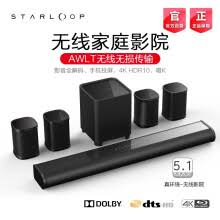
\includegraphics{/images/starloop.jpeg}
\href{https://item.jd.com/46240689641.html\#crumb-wrap}{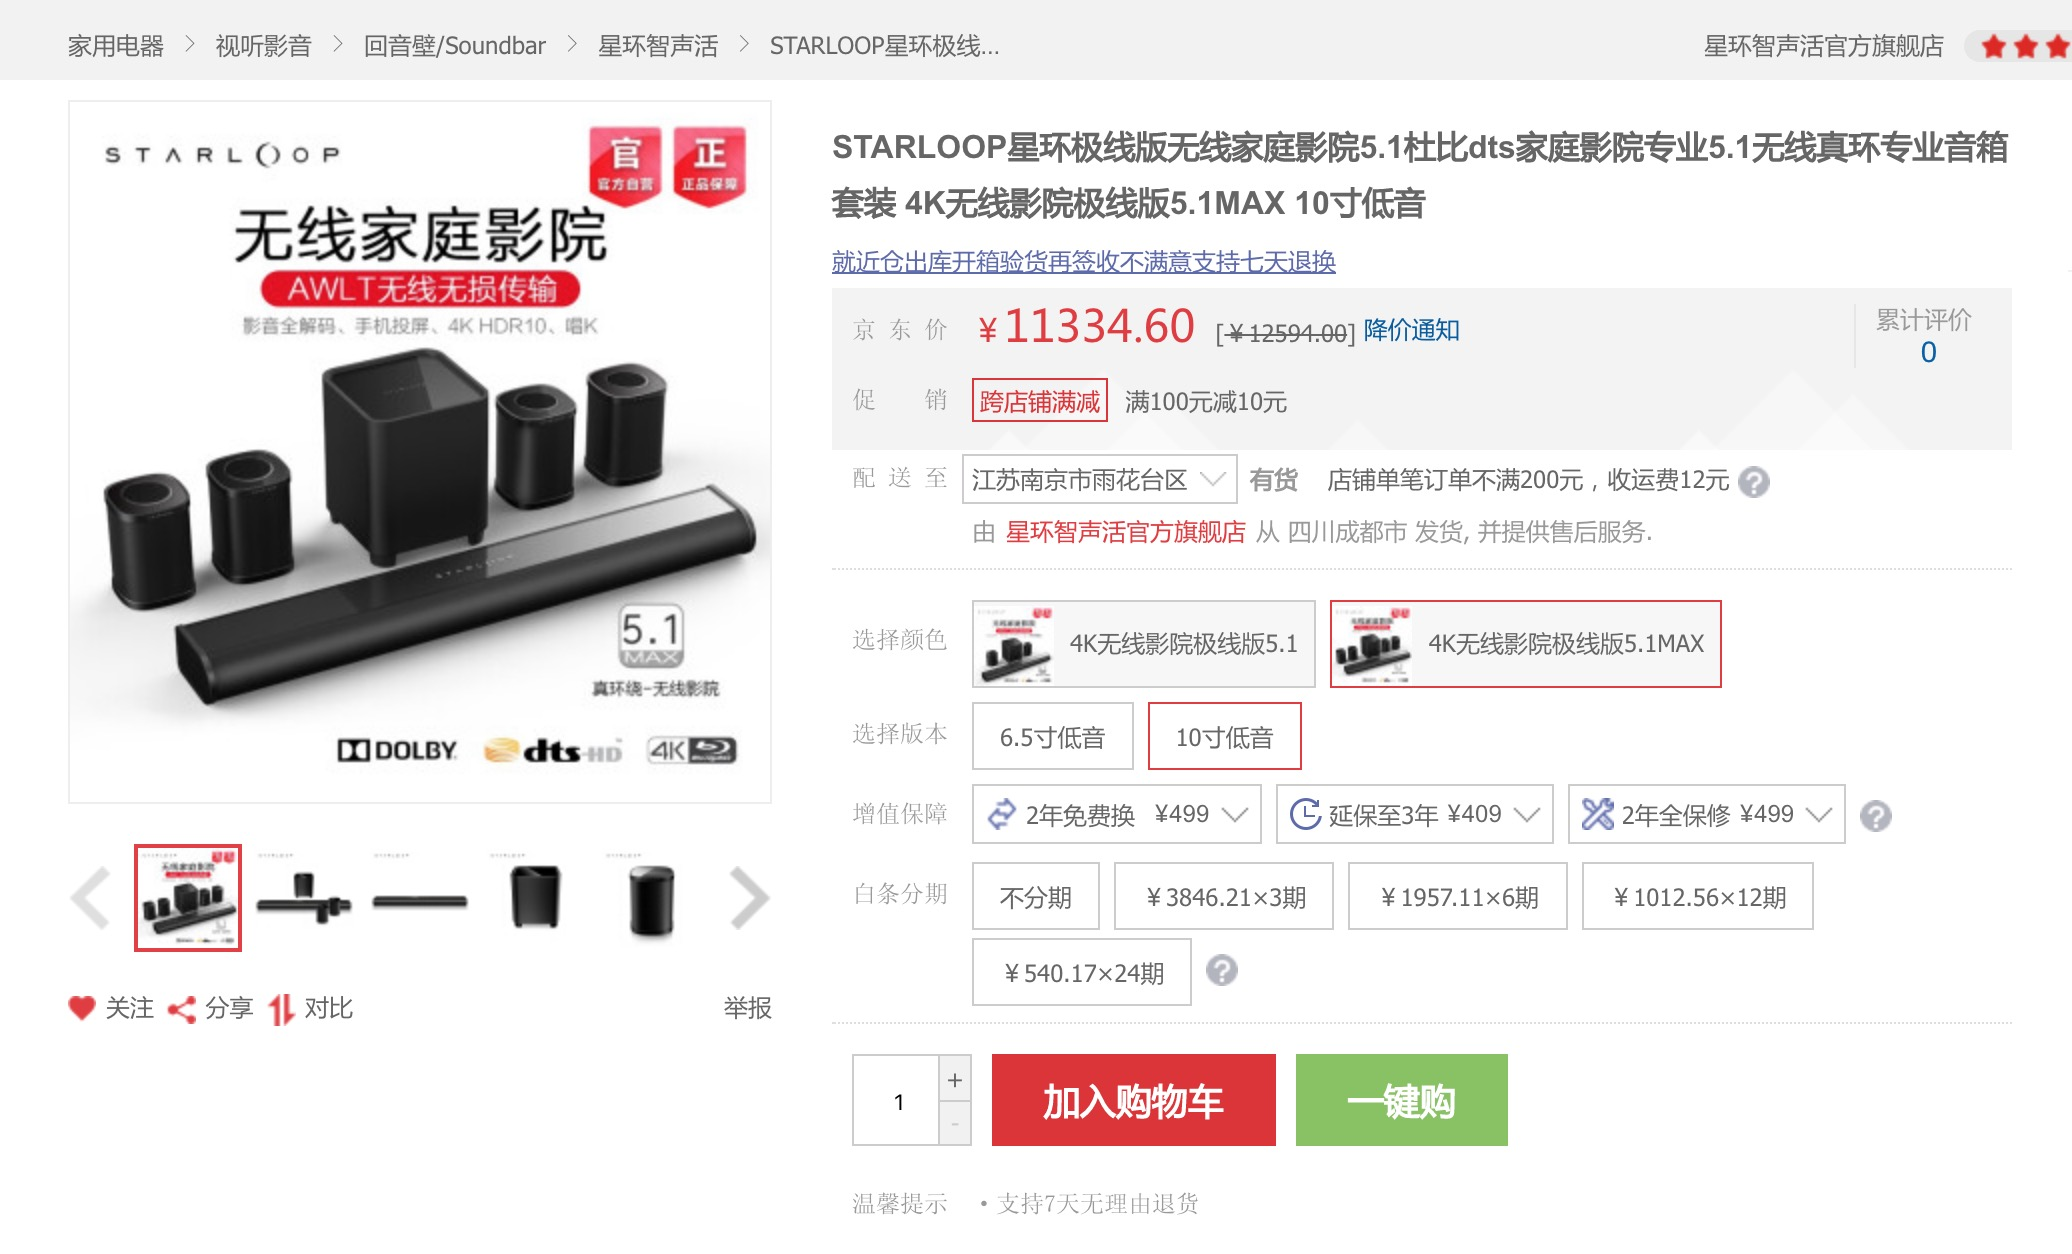
\includegraphics{/images/starloop1.jpeg}}
\href{https://item.jd.com/40250560734.html}{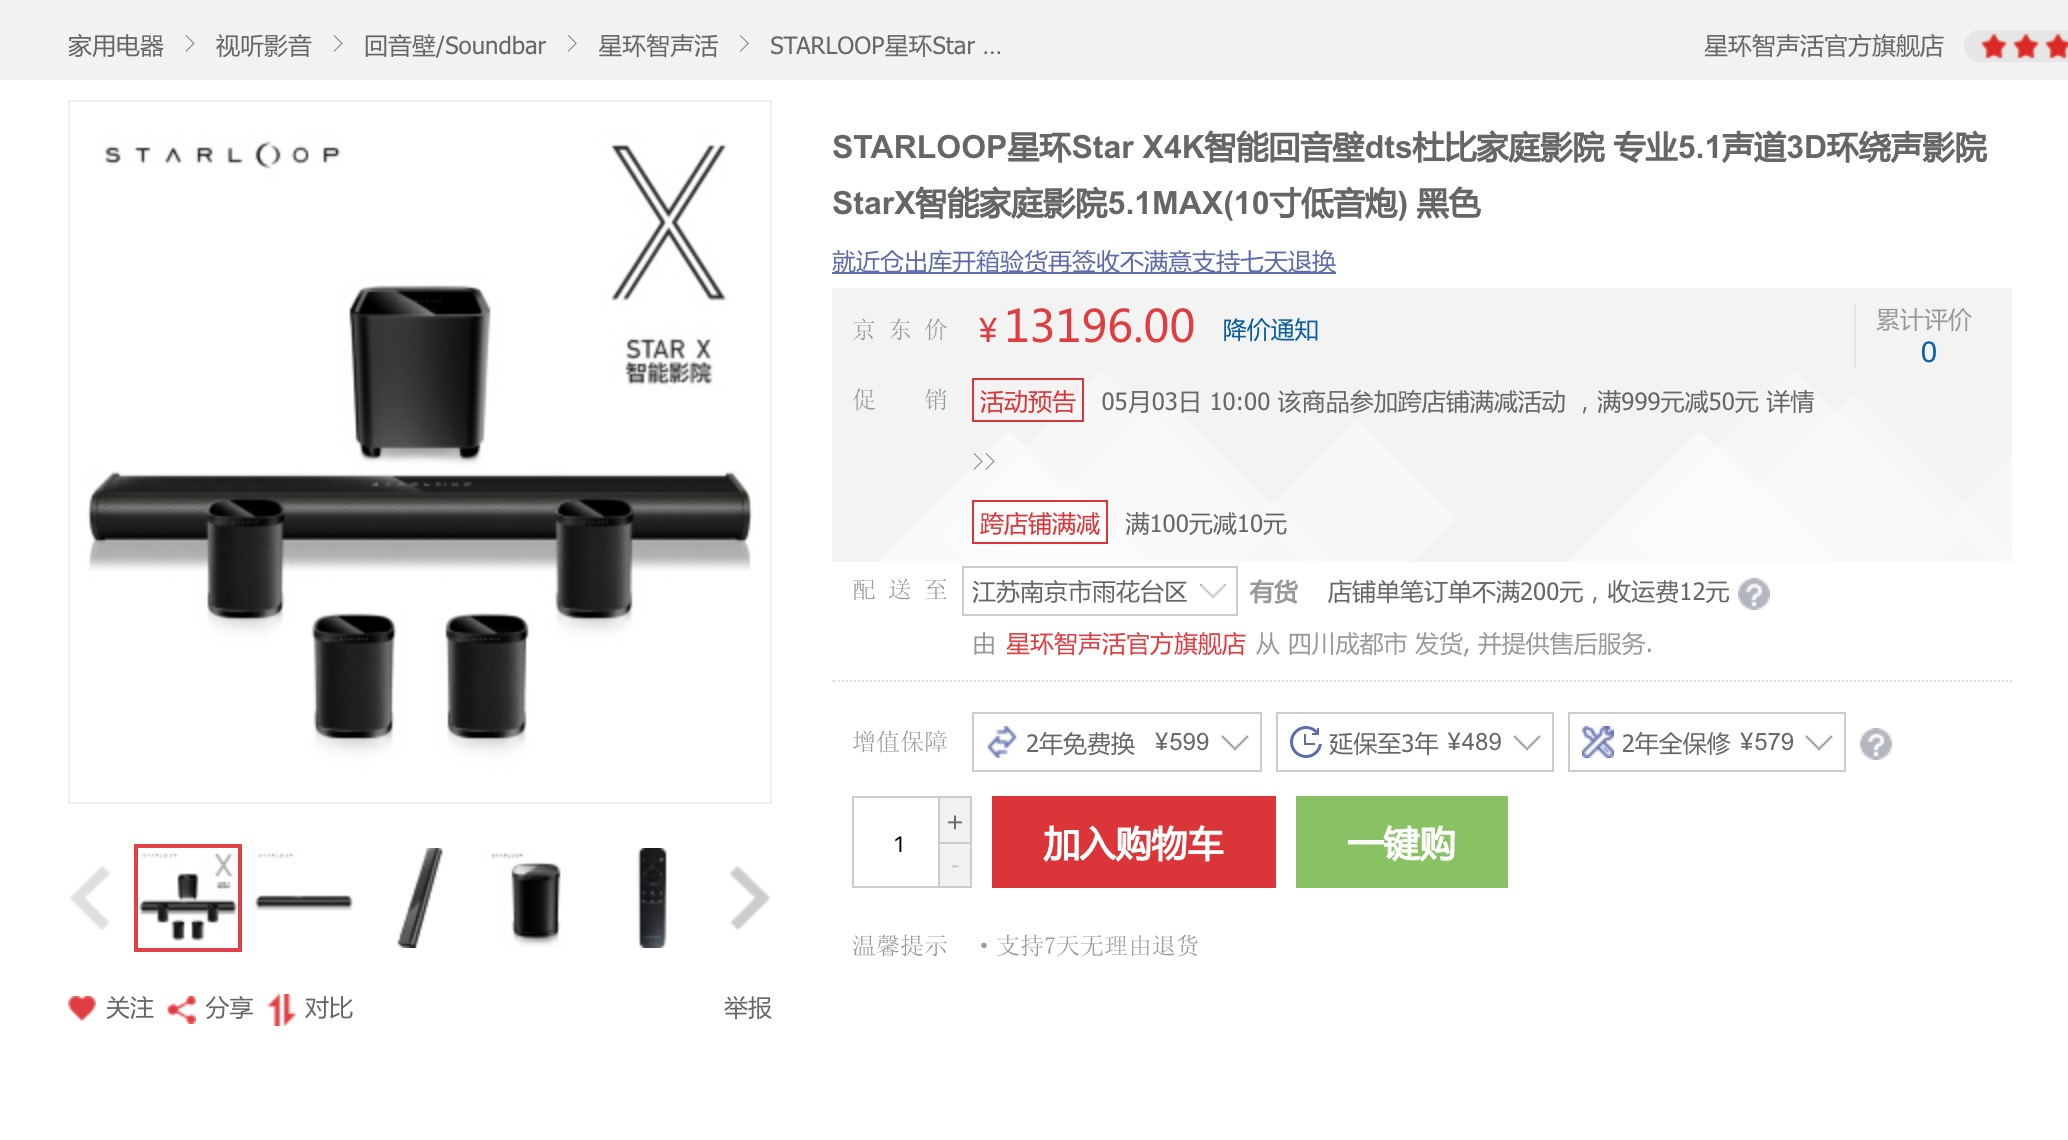
\includegraphics{/images/starloopX.jpeg}}

\paragraph{3.2 厨房电器购买}

\begin{itemize}
\tightlist
\item
  水槽
\end{itemize}

\href{https://item.taobao.com/item.htm?spm=a1z0d.6639537.1997196601.151.13307484E7ianp\&id=582513074414}{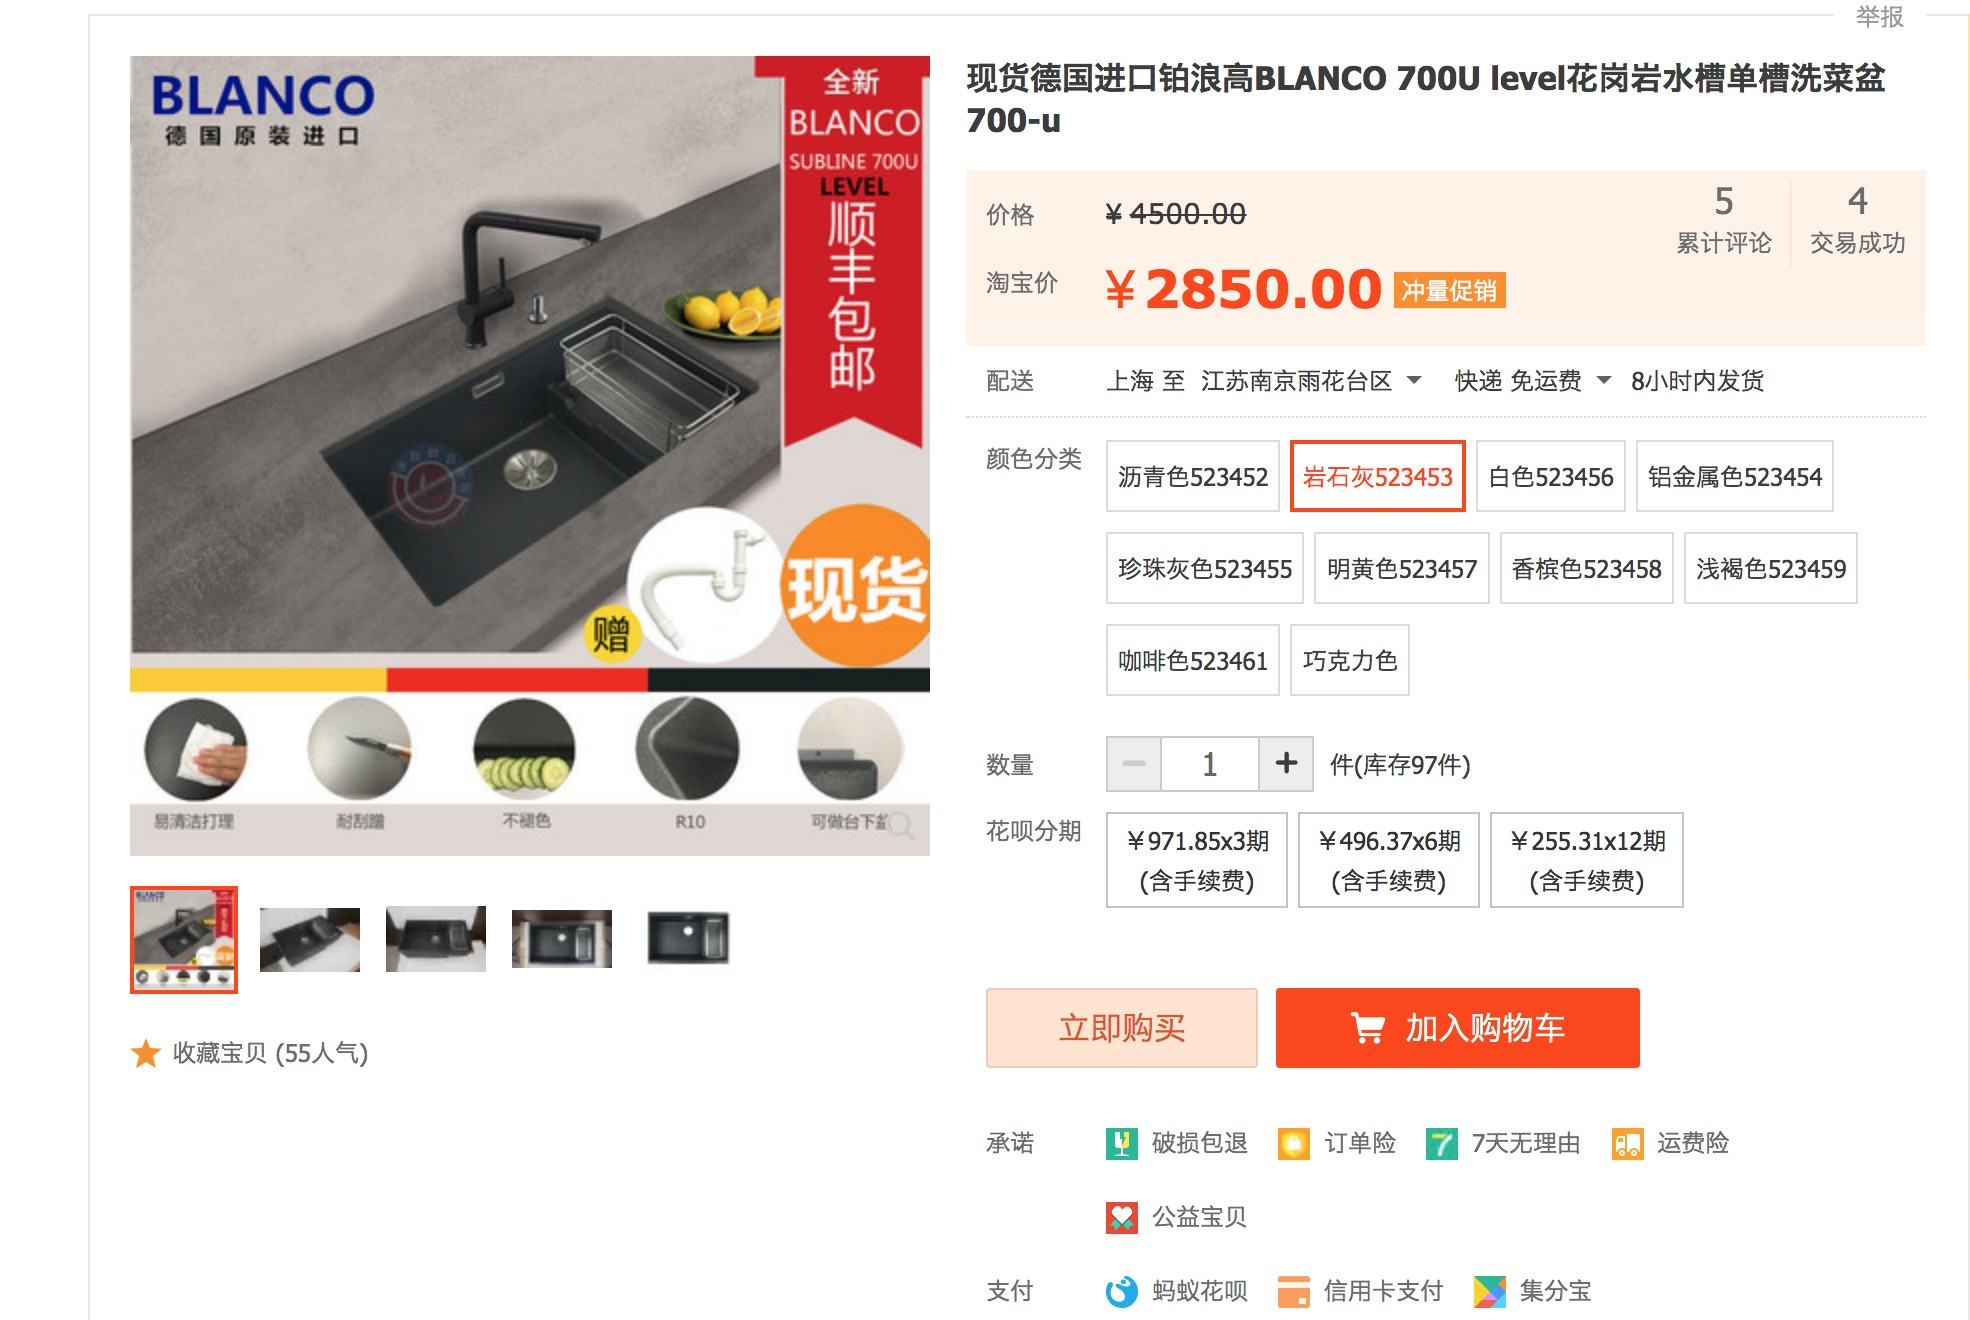
\includegraphics{/images/shuicao.jpeg}}

\begin{itemize}
\tightlist
\item
  燃气灶+油烟机
\end{itemize}

\href{https://item.jd.com/2607373.html\#crumb-wrap}{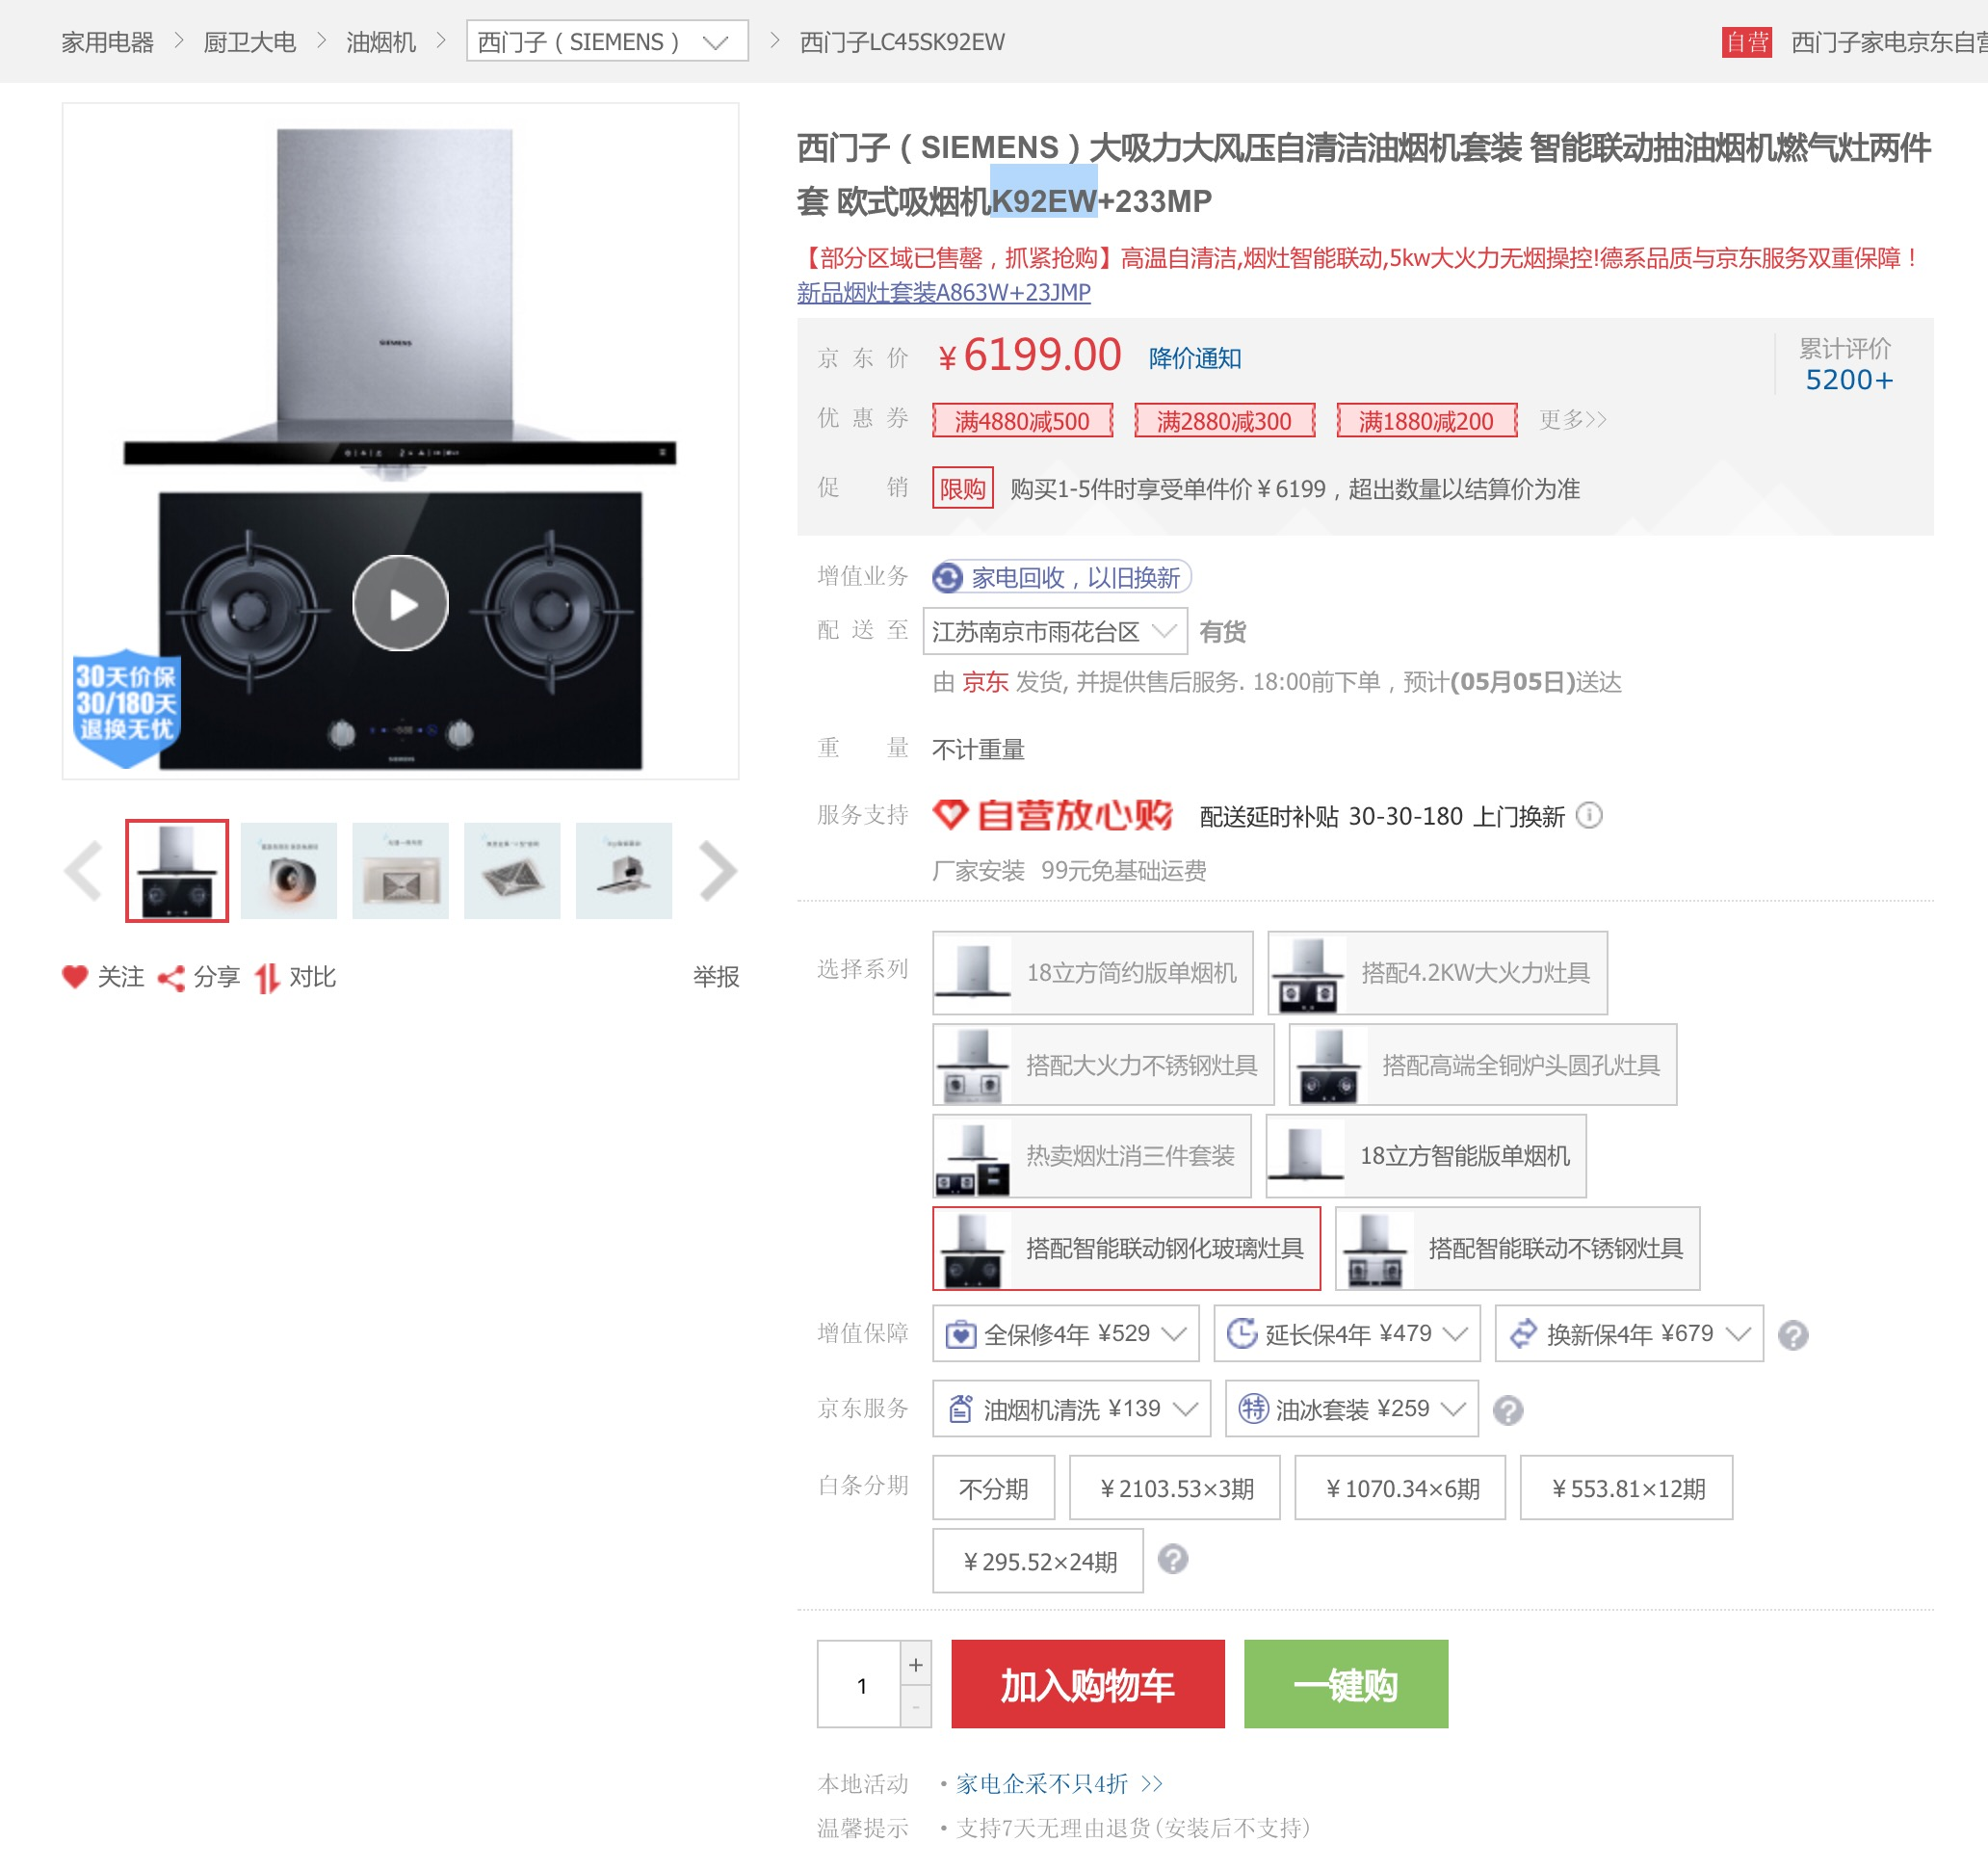
\includegraphics{/images/youyanji1.jpeg}}

\href{https://item.jd.com/100003279296.html}{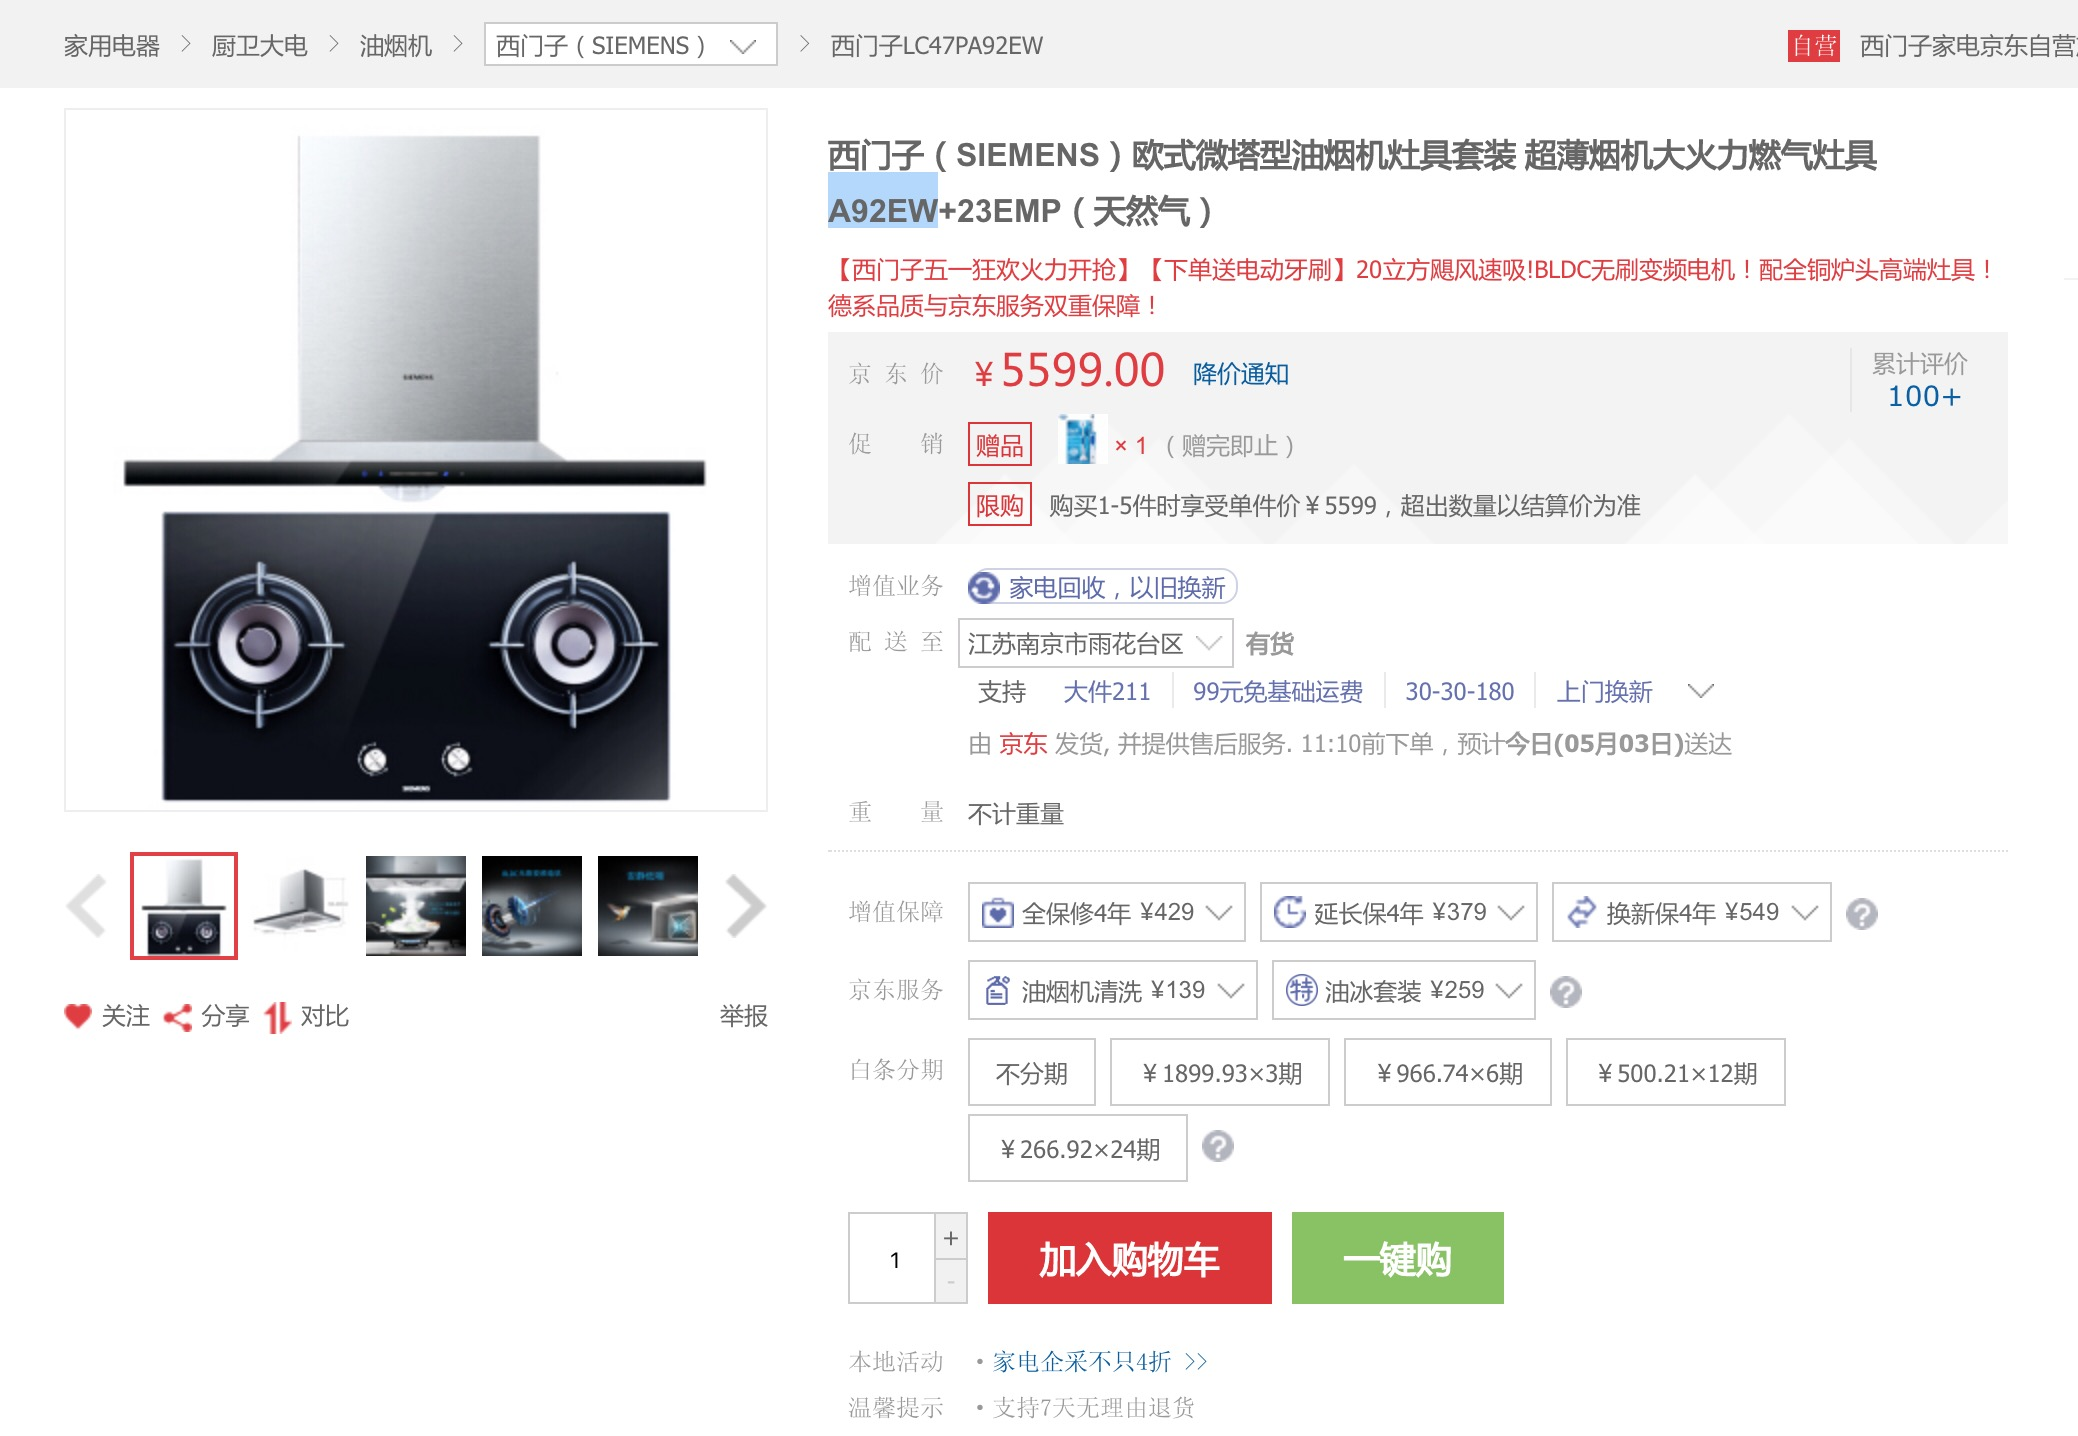
\includegraphics{/images/youyanji2.jpeg}}

\begin{itemize}
\tightlist
\item
  洗碗机:\href{https://post.smzdm.com/p/a25rq6rp/}{下面两款评测对比}
\end{itemize}

\href{https://item.jd.com/100004828676.html}{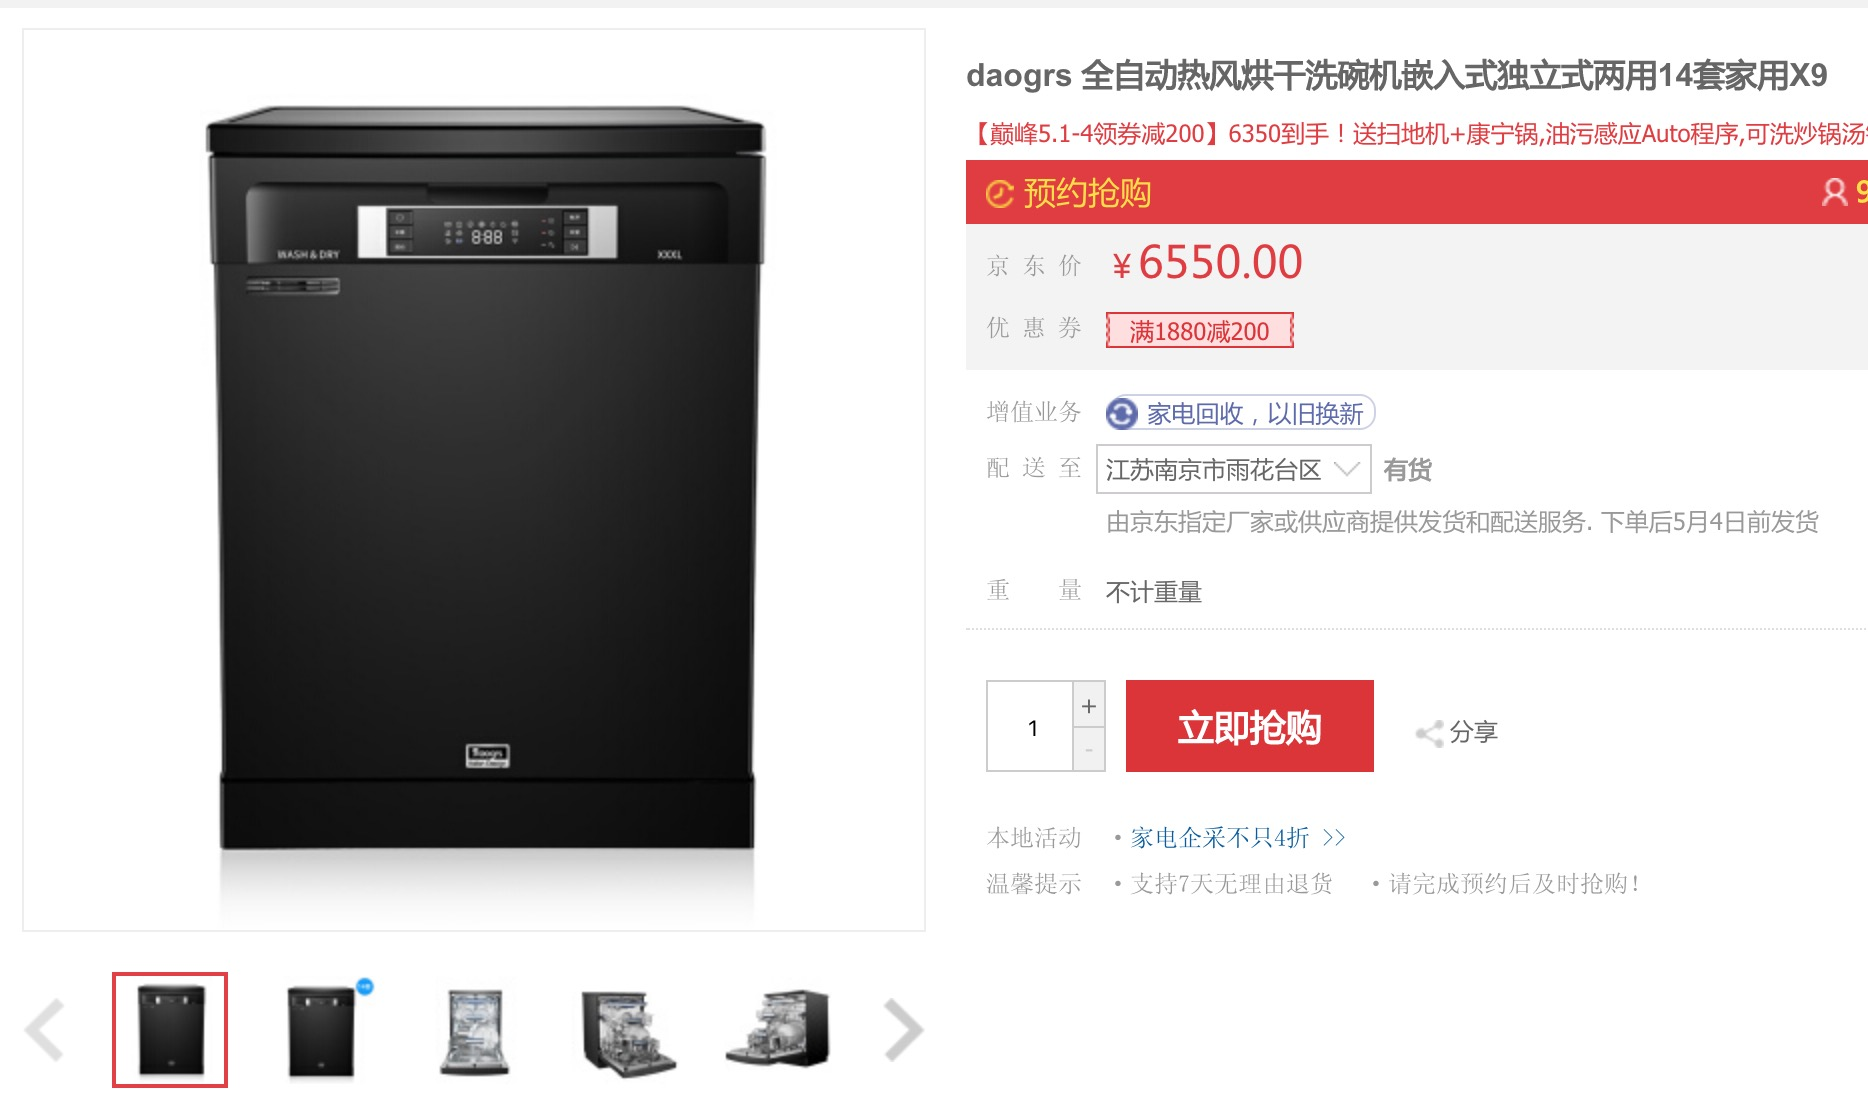
\includegraphics{/images/xiwanji-daogrs1.jpeg}}

\href{https://item.jd.com/11289763170.html}{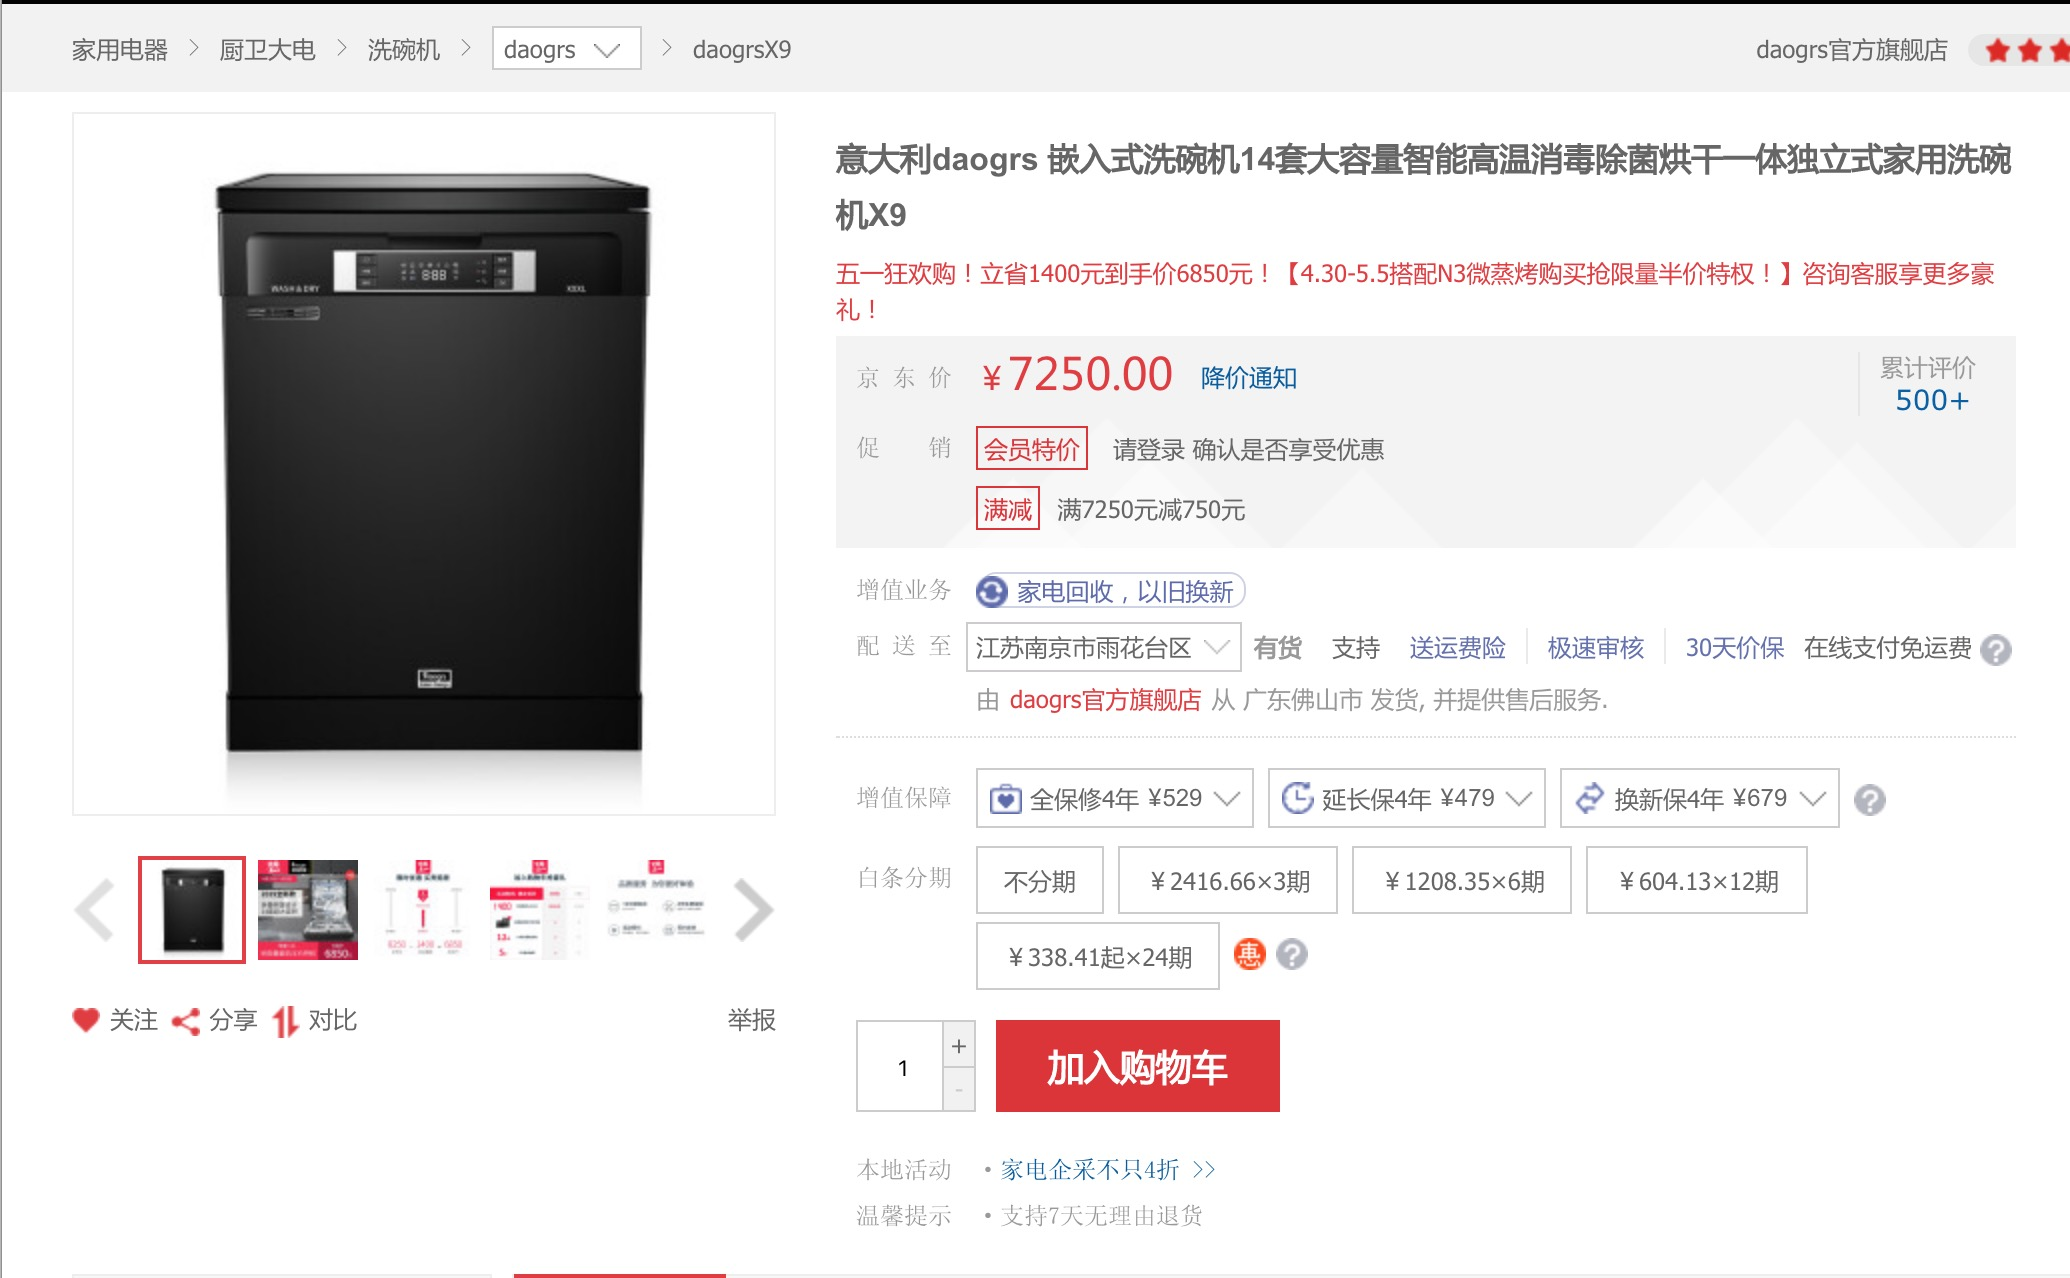
\includegraphics{/images/xiwanji-daogrs2.jpeg}}
\href{https://item.jd.com/7214578.html\#crumb-wrap}{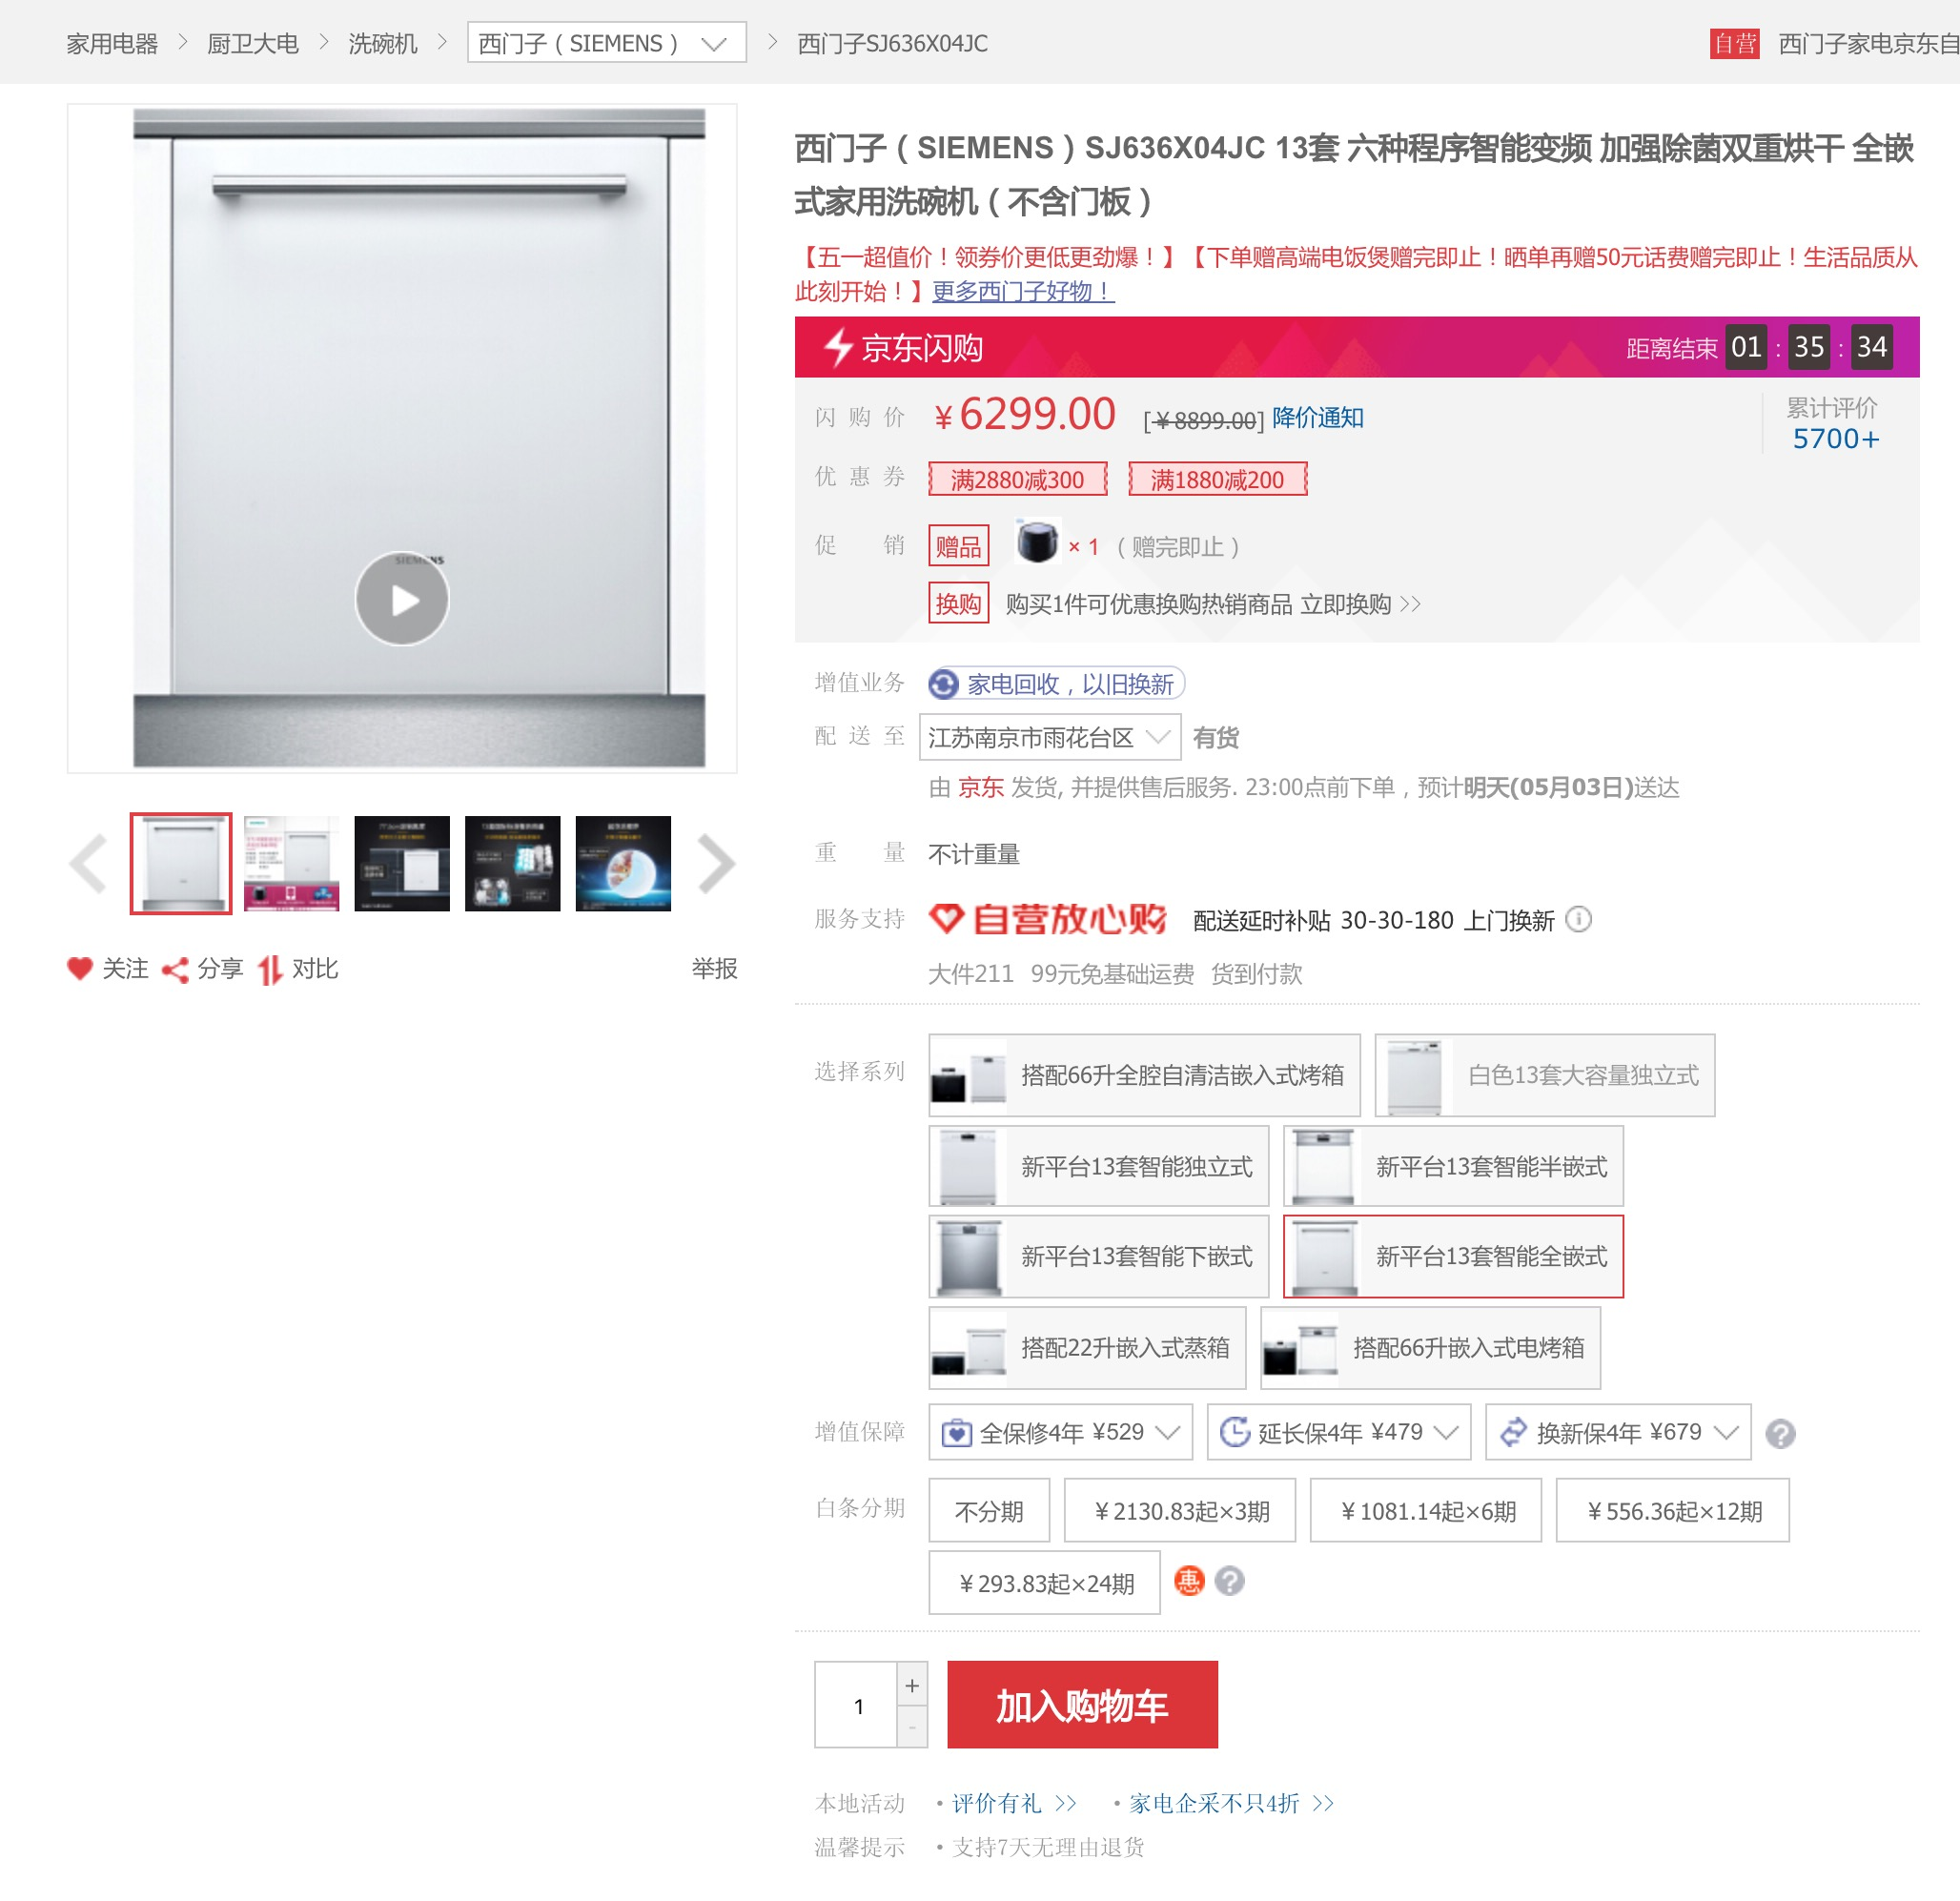
\includegraphics{/images/xiwanji-simens1.jpeg}}
\href{https://item.jd.com/7428417.html}{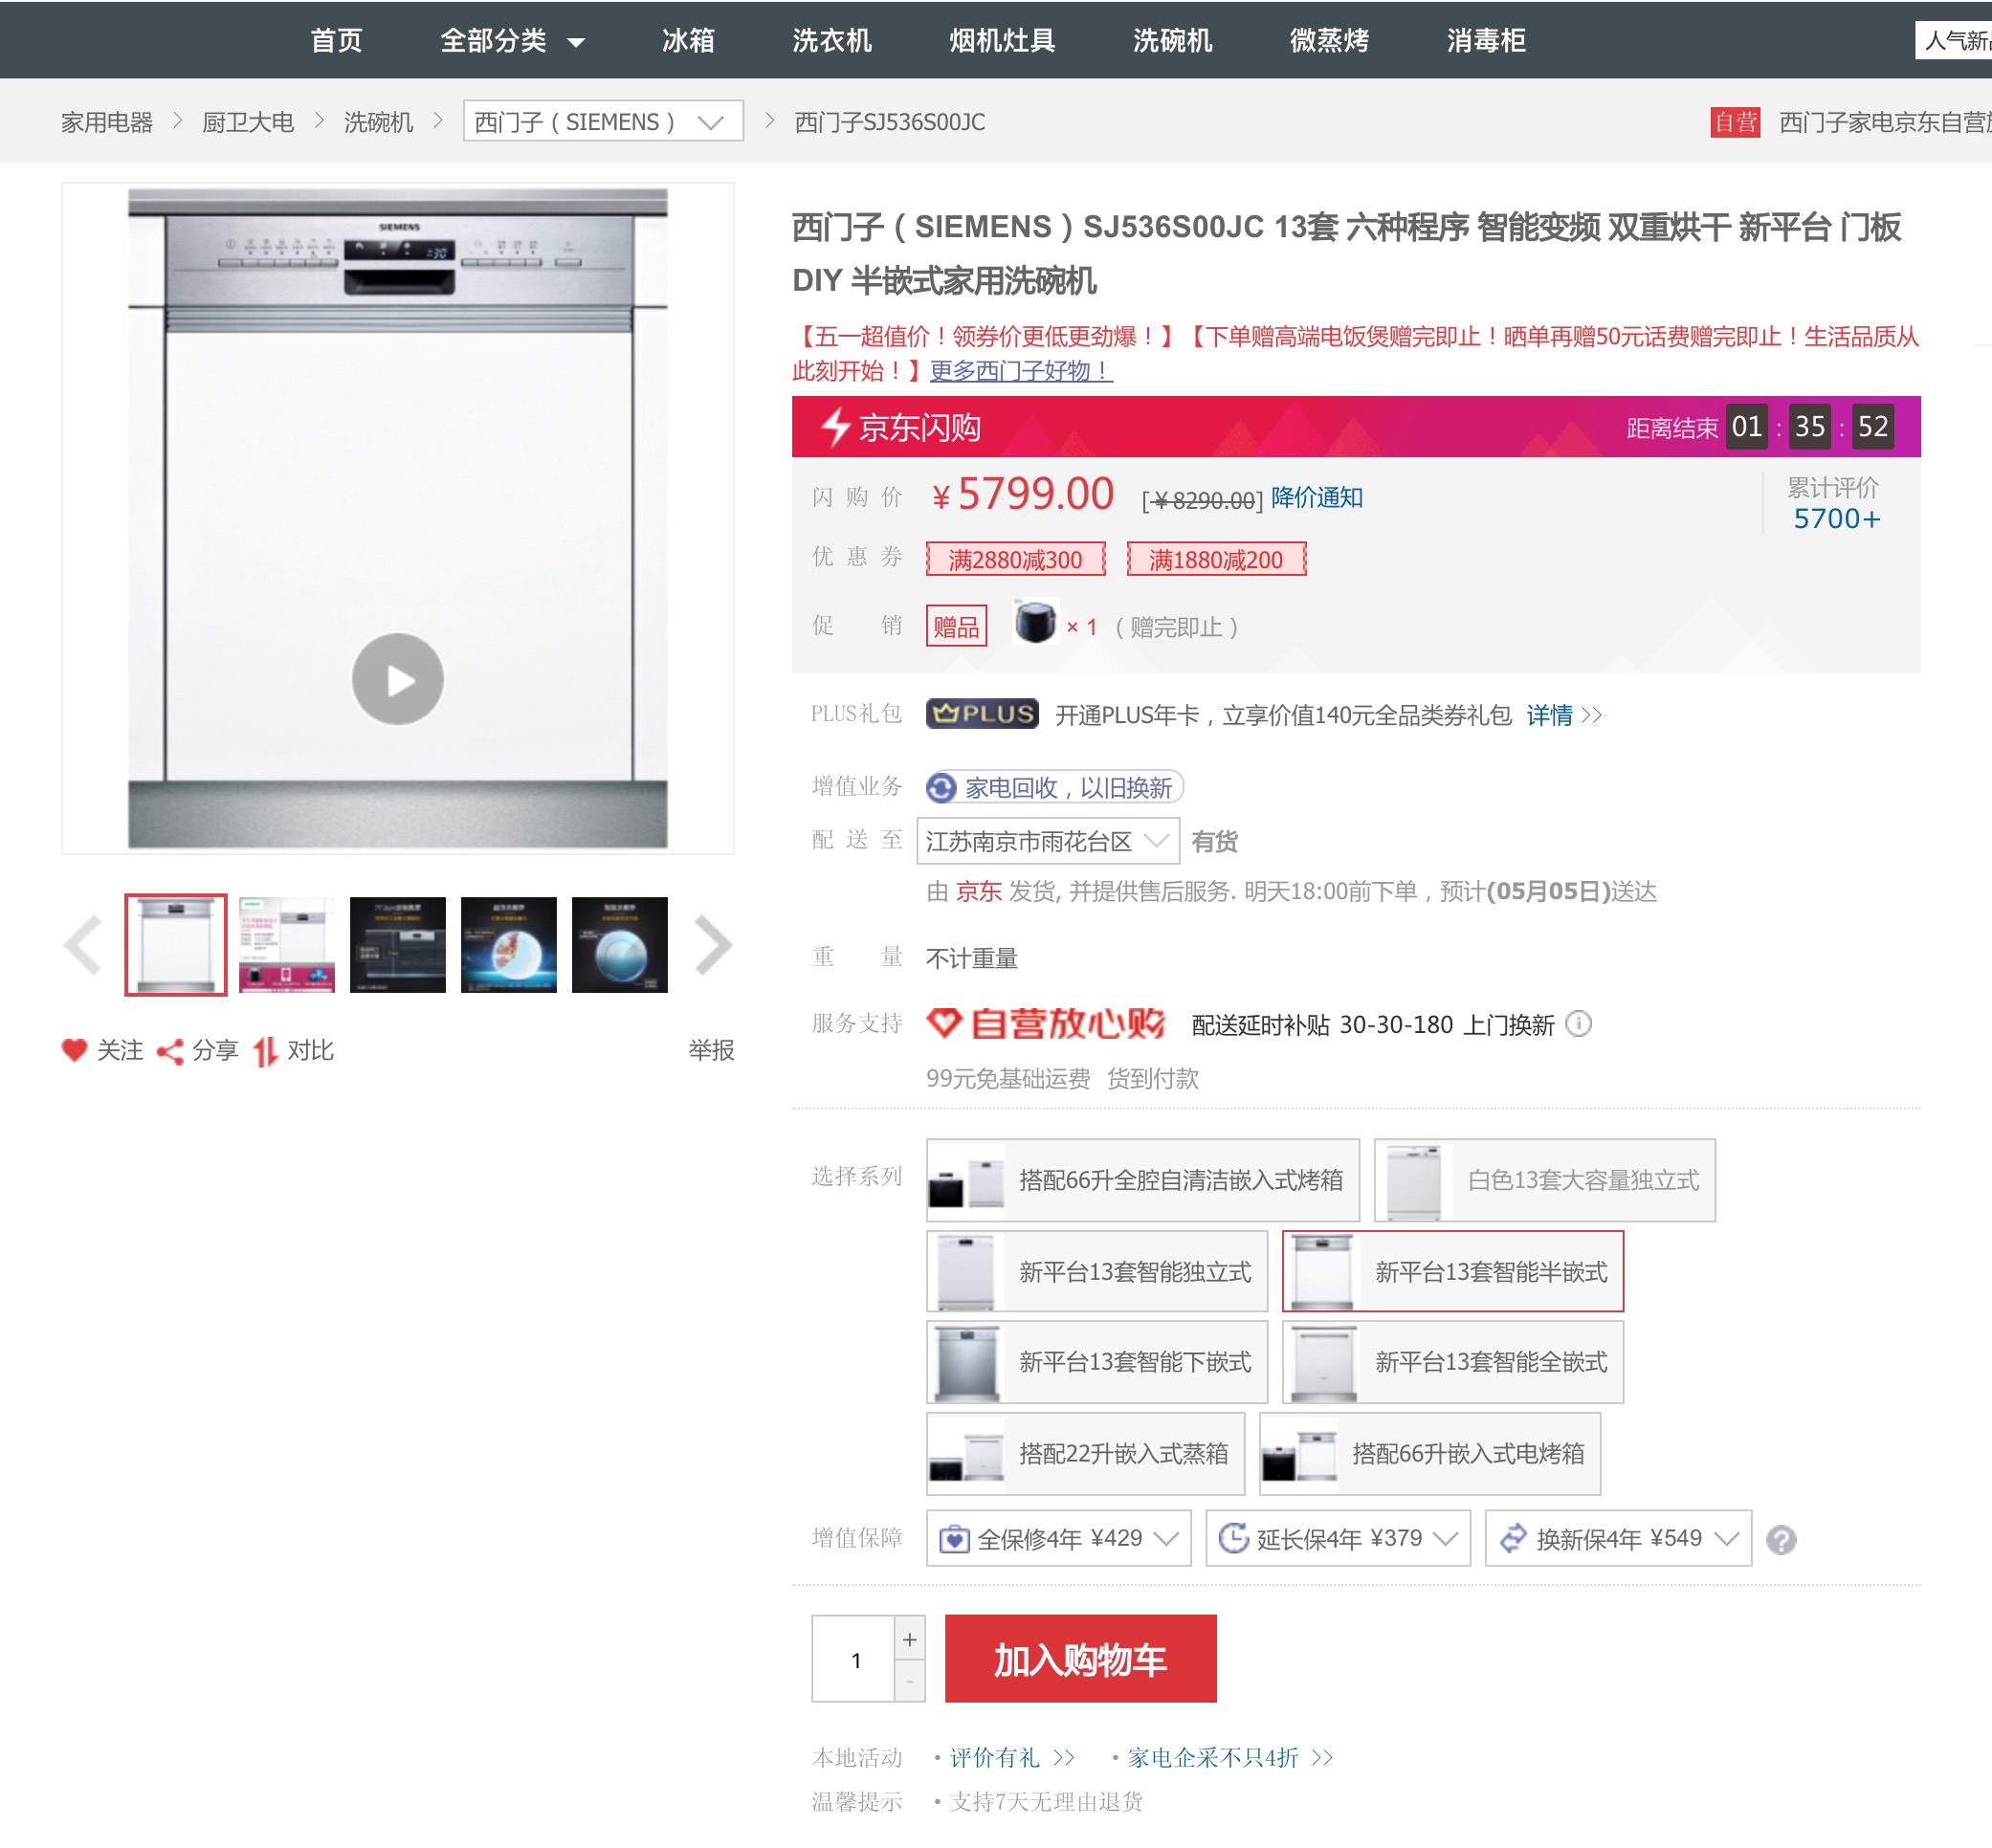
\includegraphics{/images/xiwanji-simens2.jpeg}}

\begin{itemize}
\tightlist
\item
  烤箱、蒸箱、微波炉
\end{itemize}

\href{https://item.jd.com/40818575852.html}{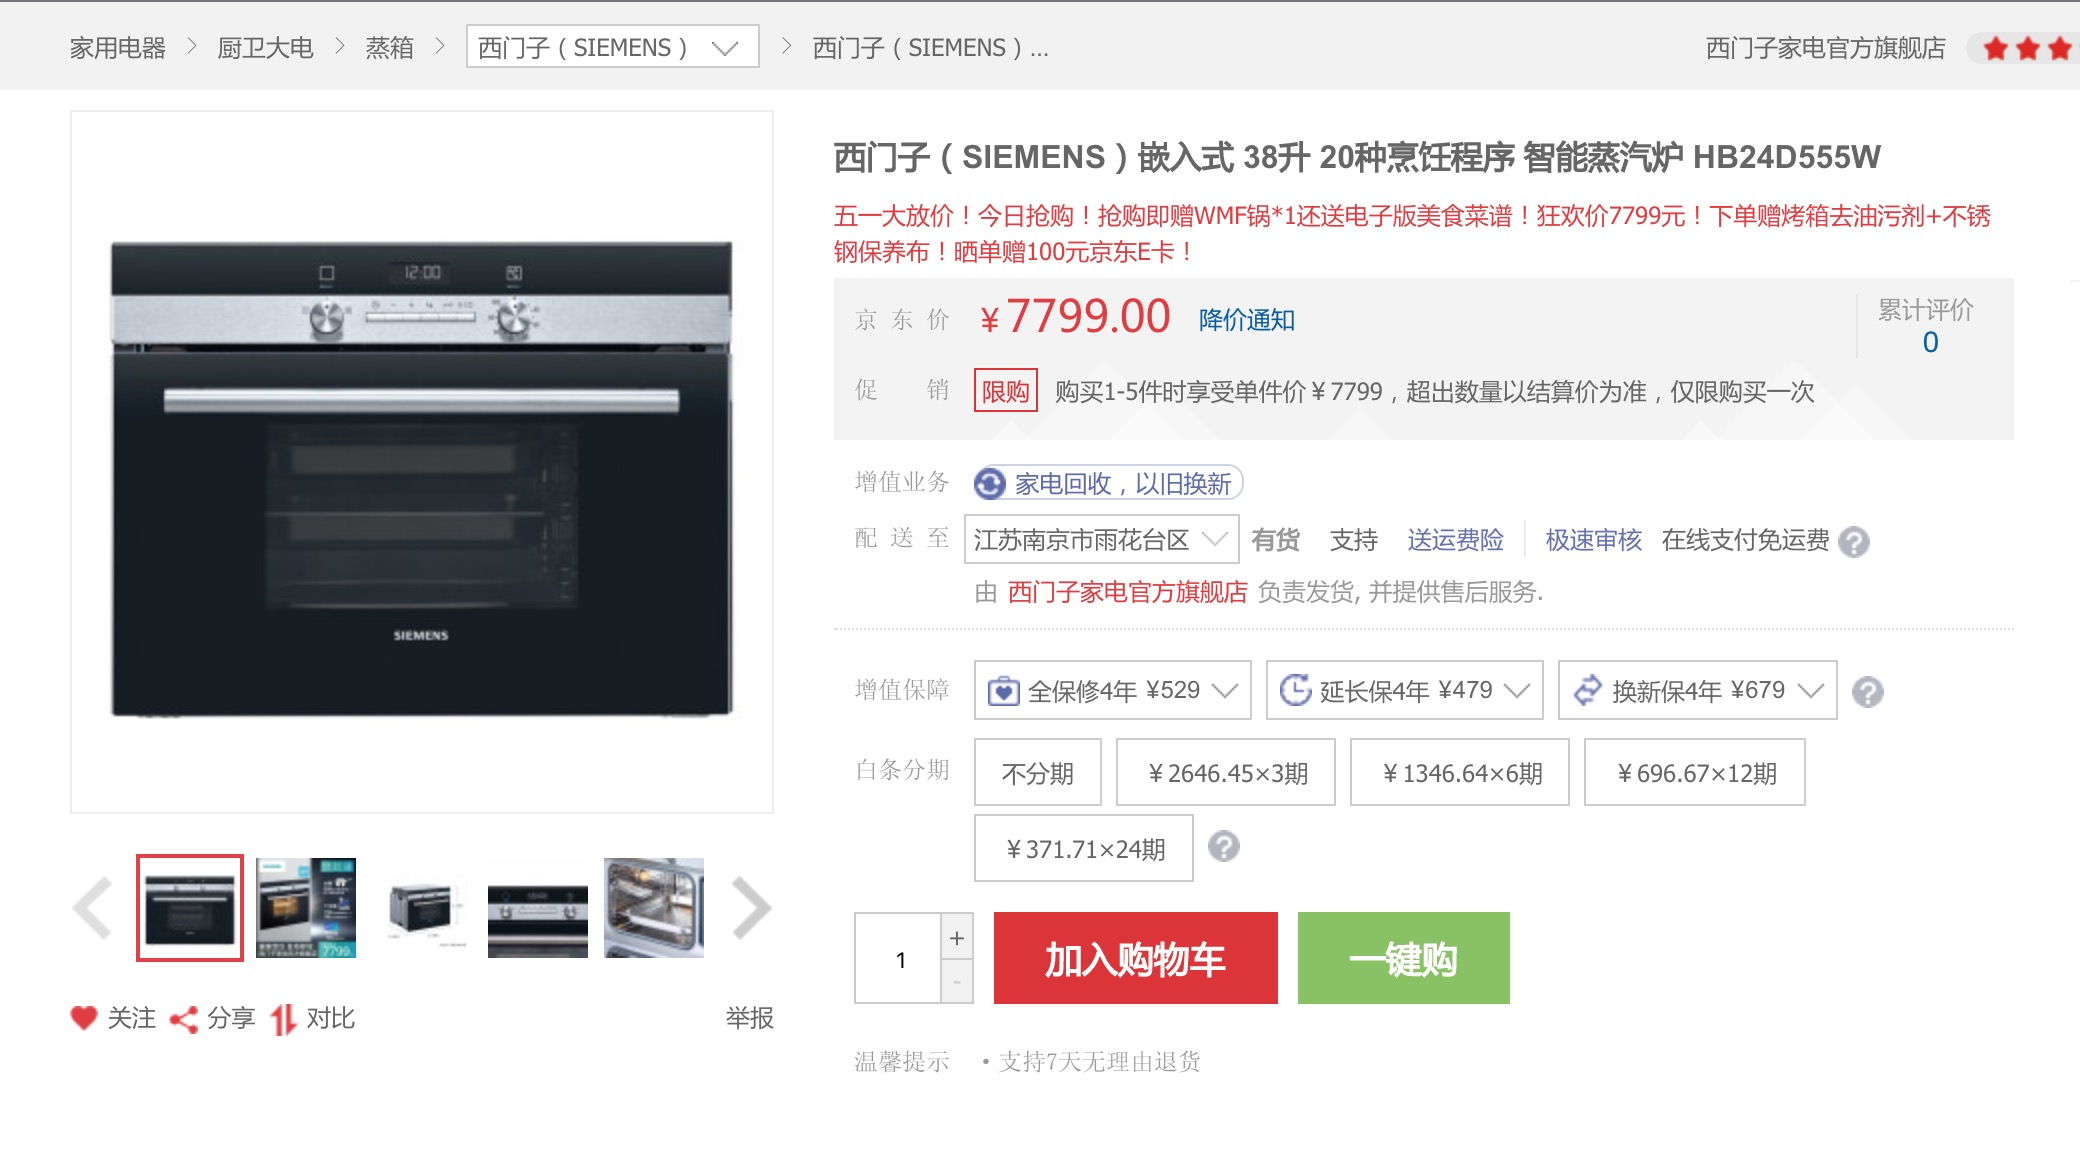
\includegraphics{/images/kaoxiang-simens1.jpeg}}
\href{https://item.jd.com/40816636872.html}{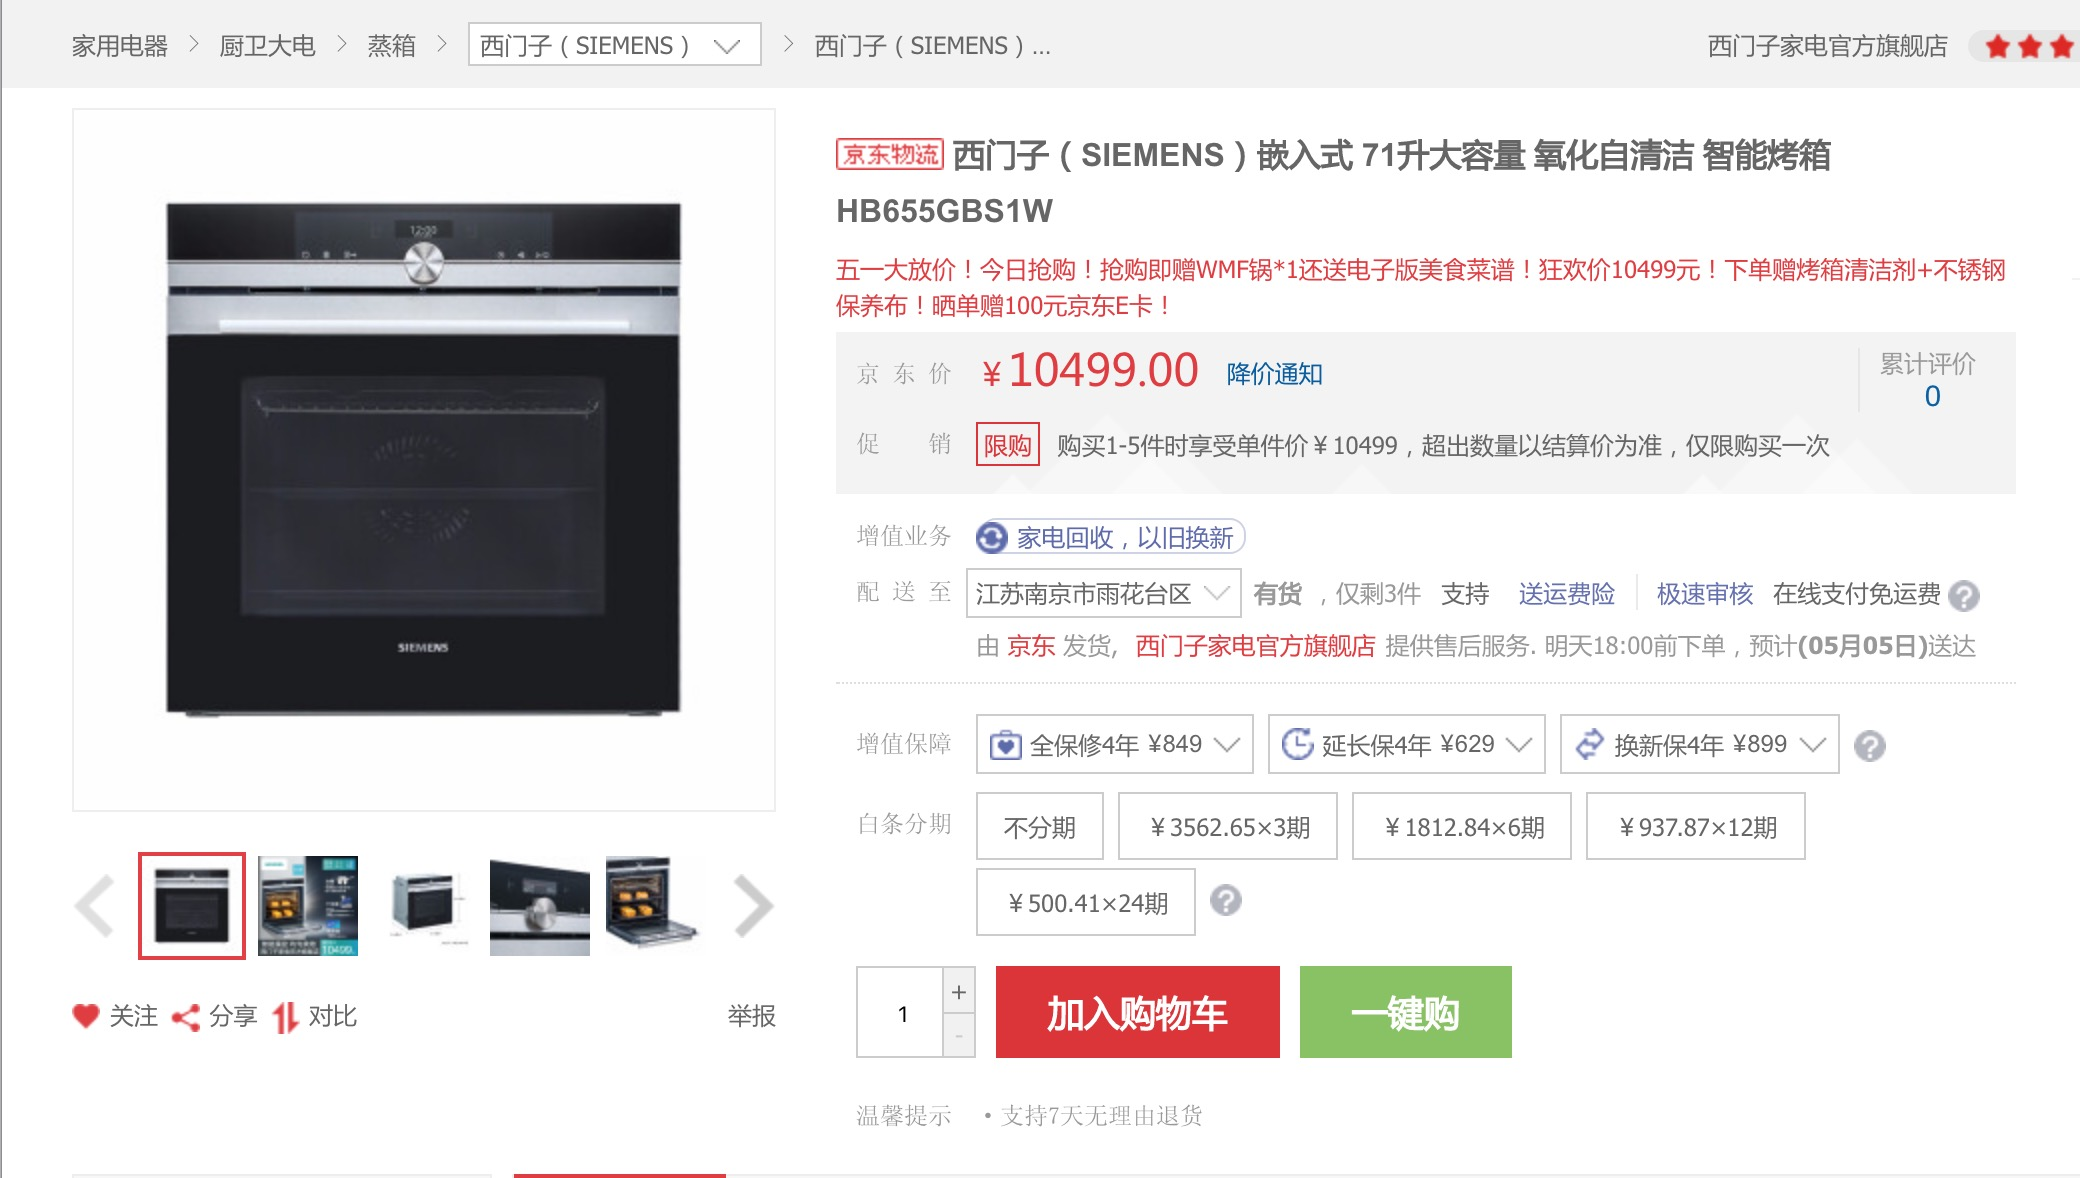
\includegraphics{/images/kaoxiang-simens2.jpeg}}
\href{https://item.jd.com/6771295.html\#crumb-wrap}{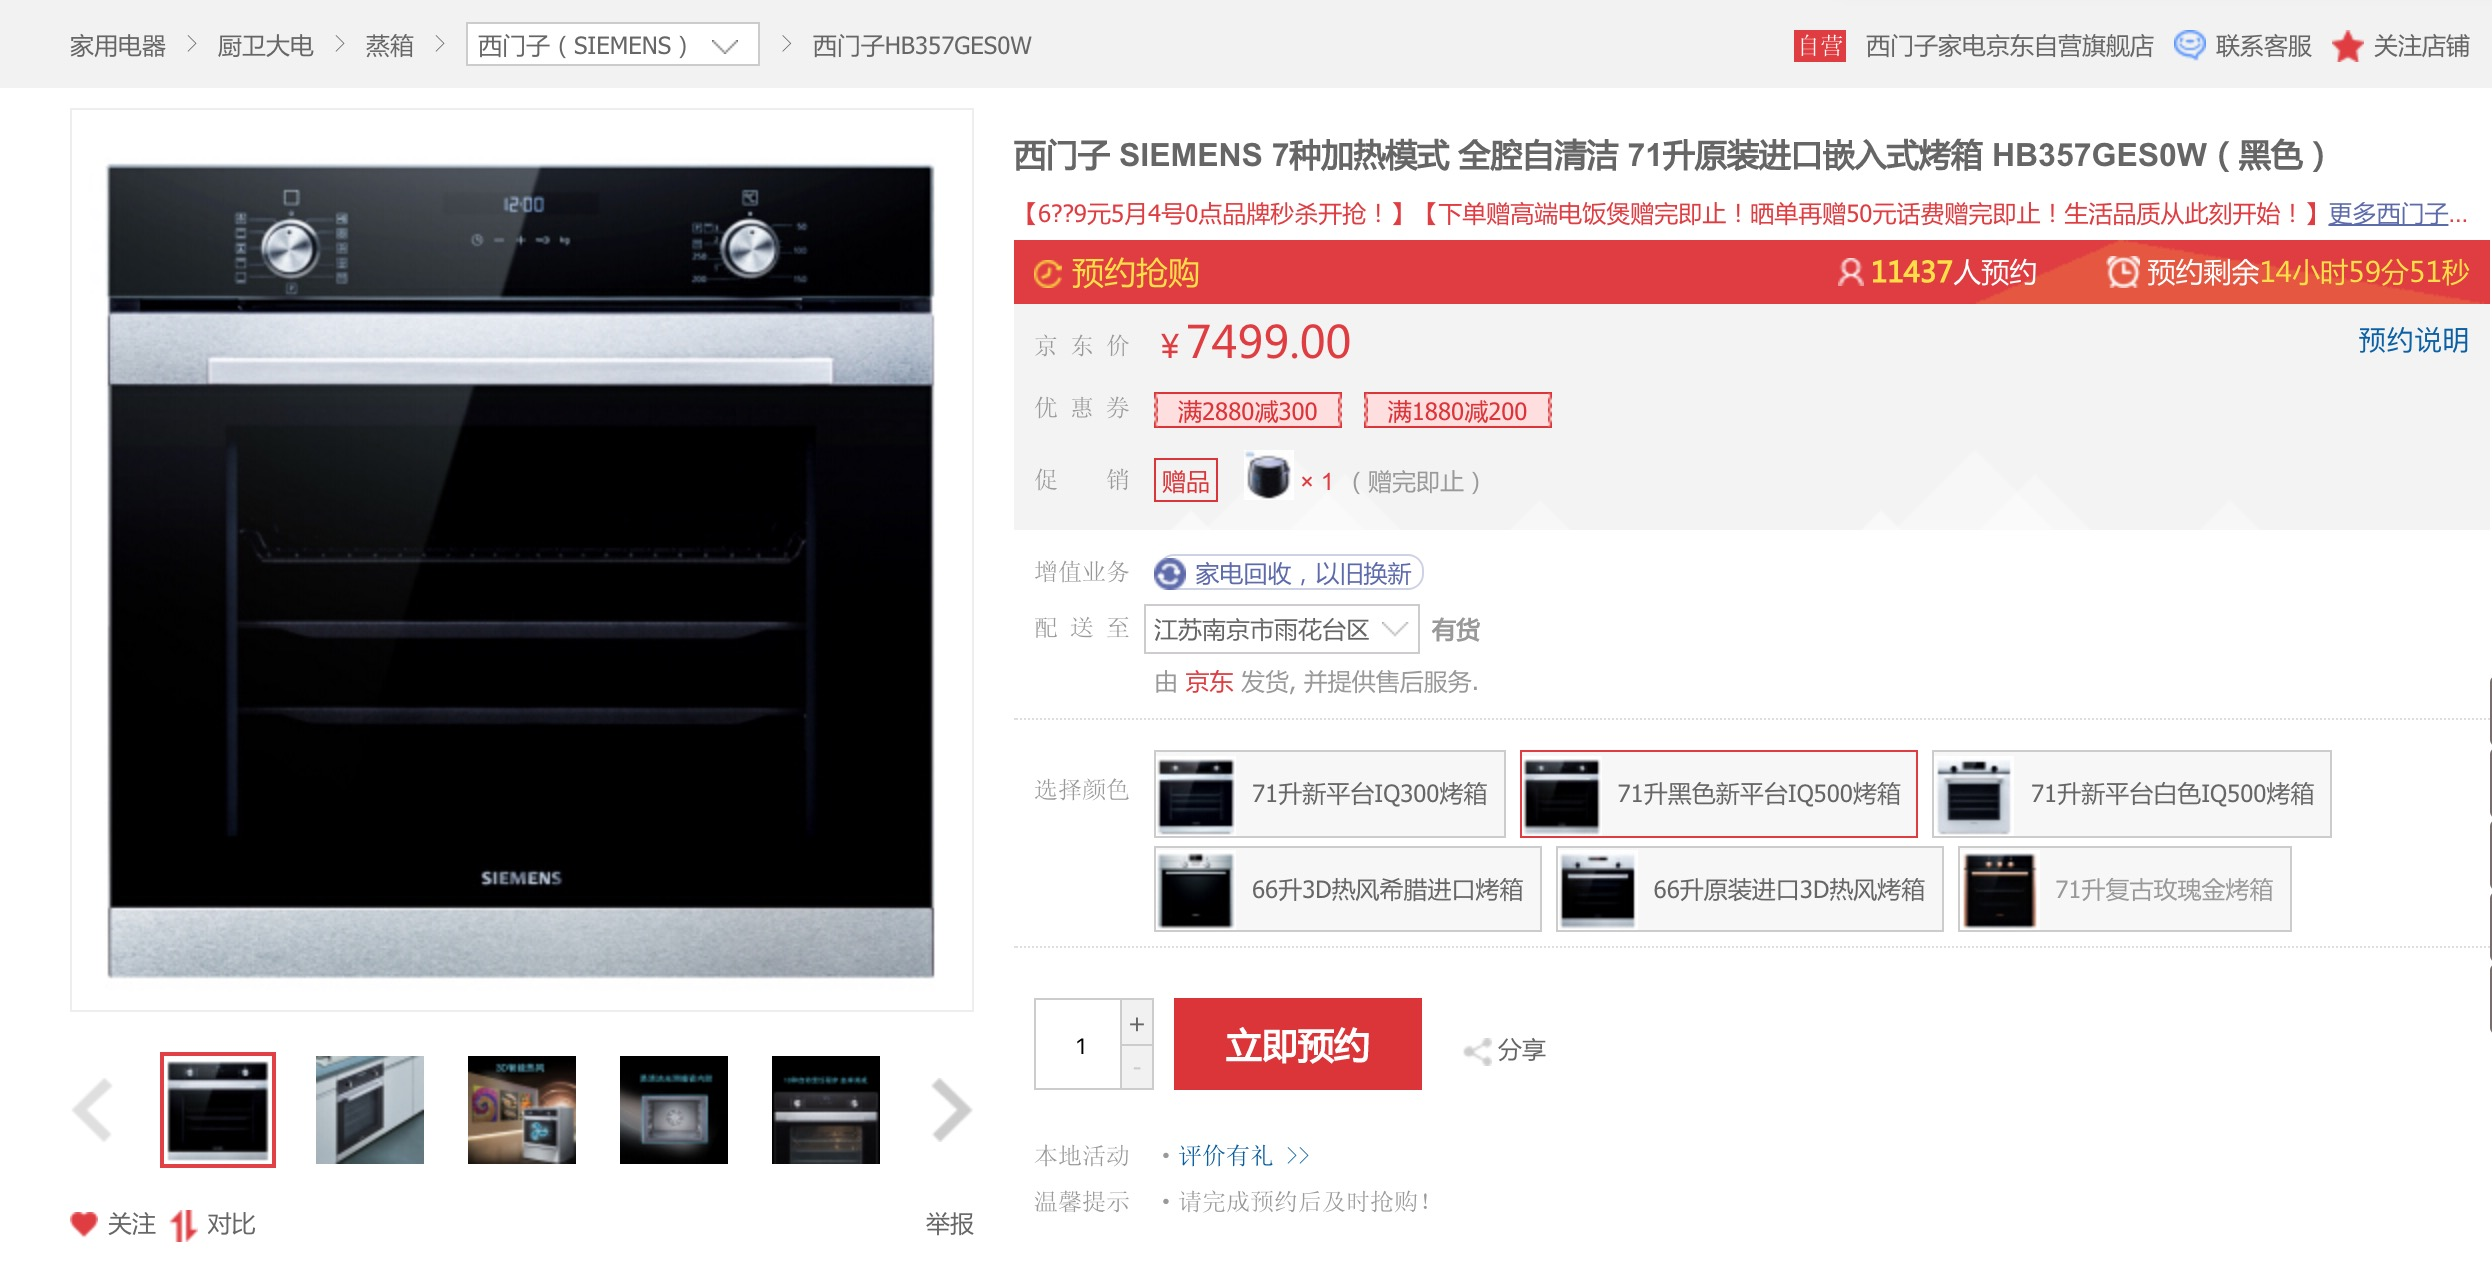
\includegraphics{/images/kaoxinag-simens21.jpeg}}
\href{https://item.jd.com/6864319.html\#crumb-wrap}{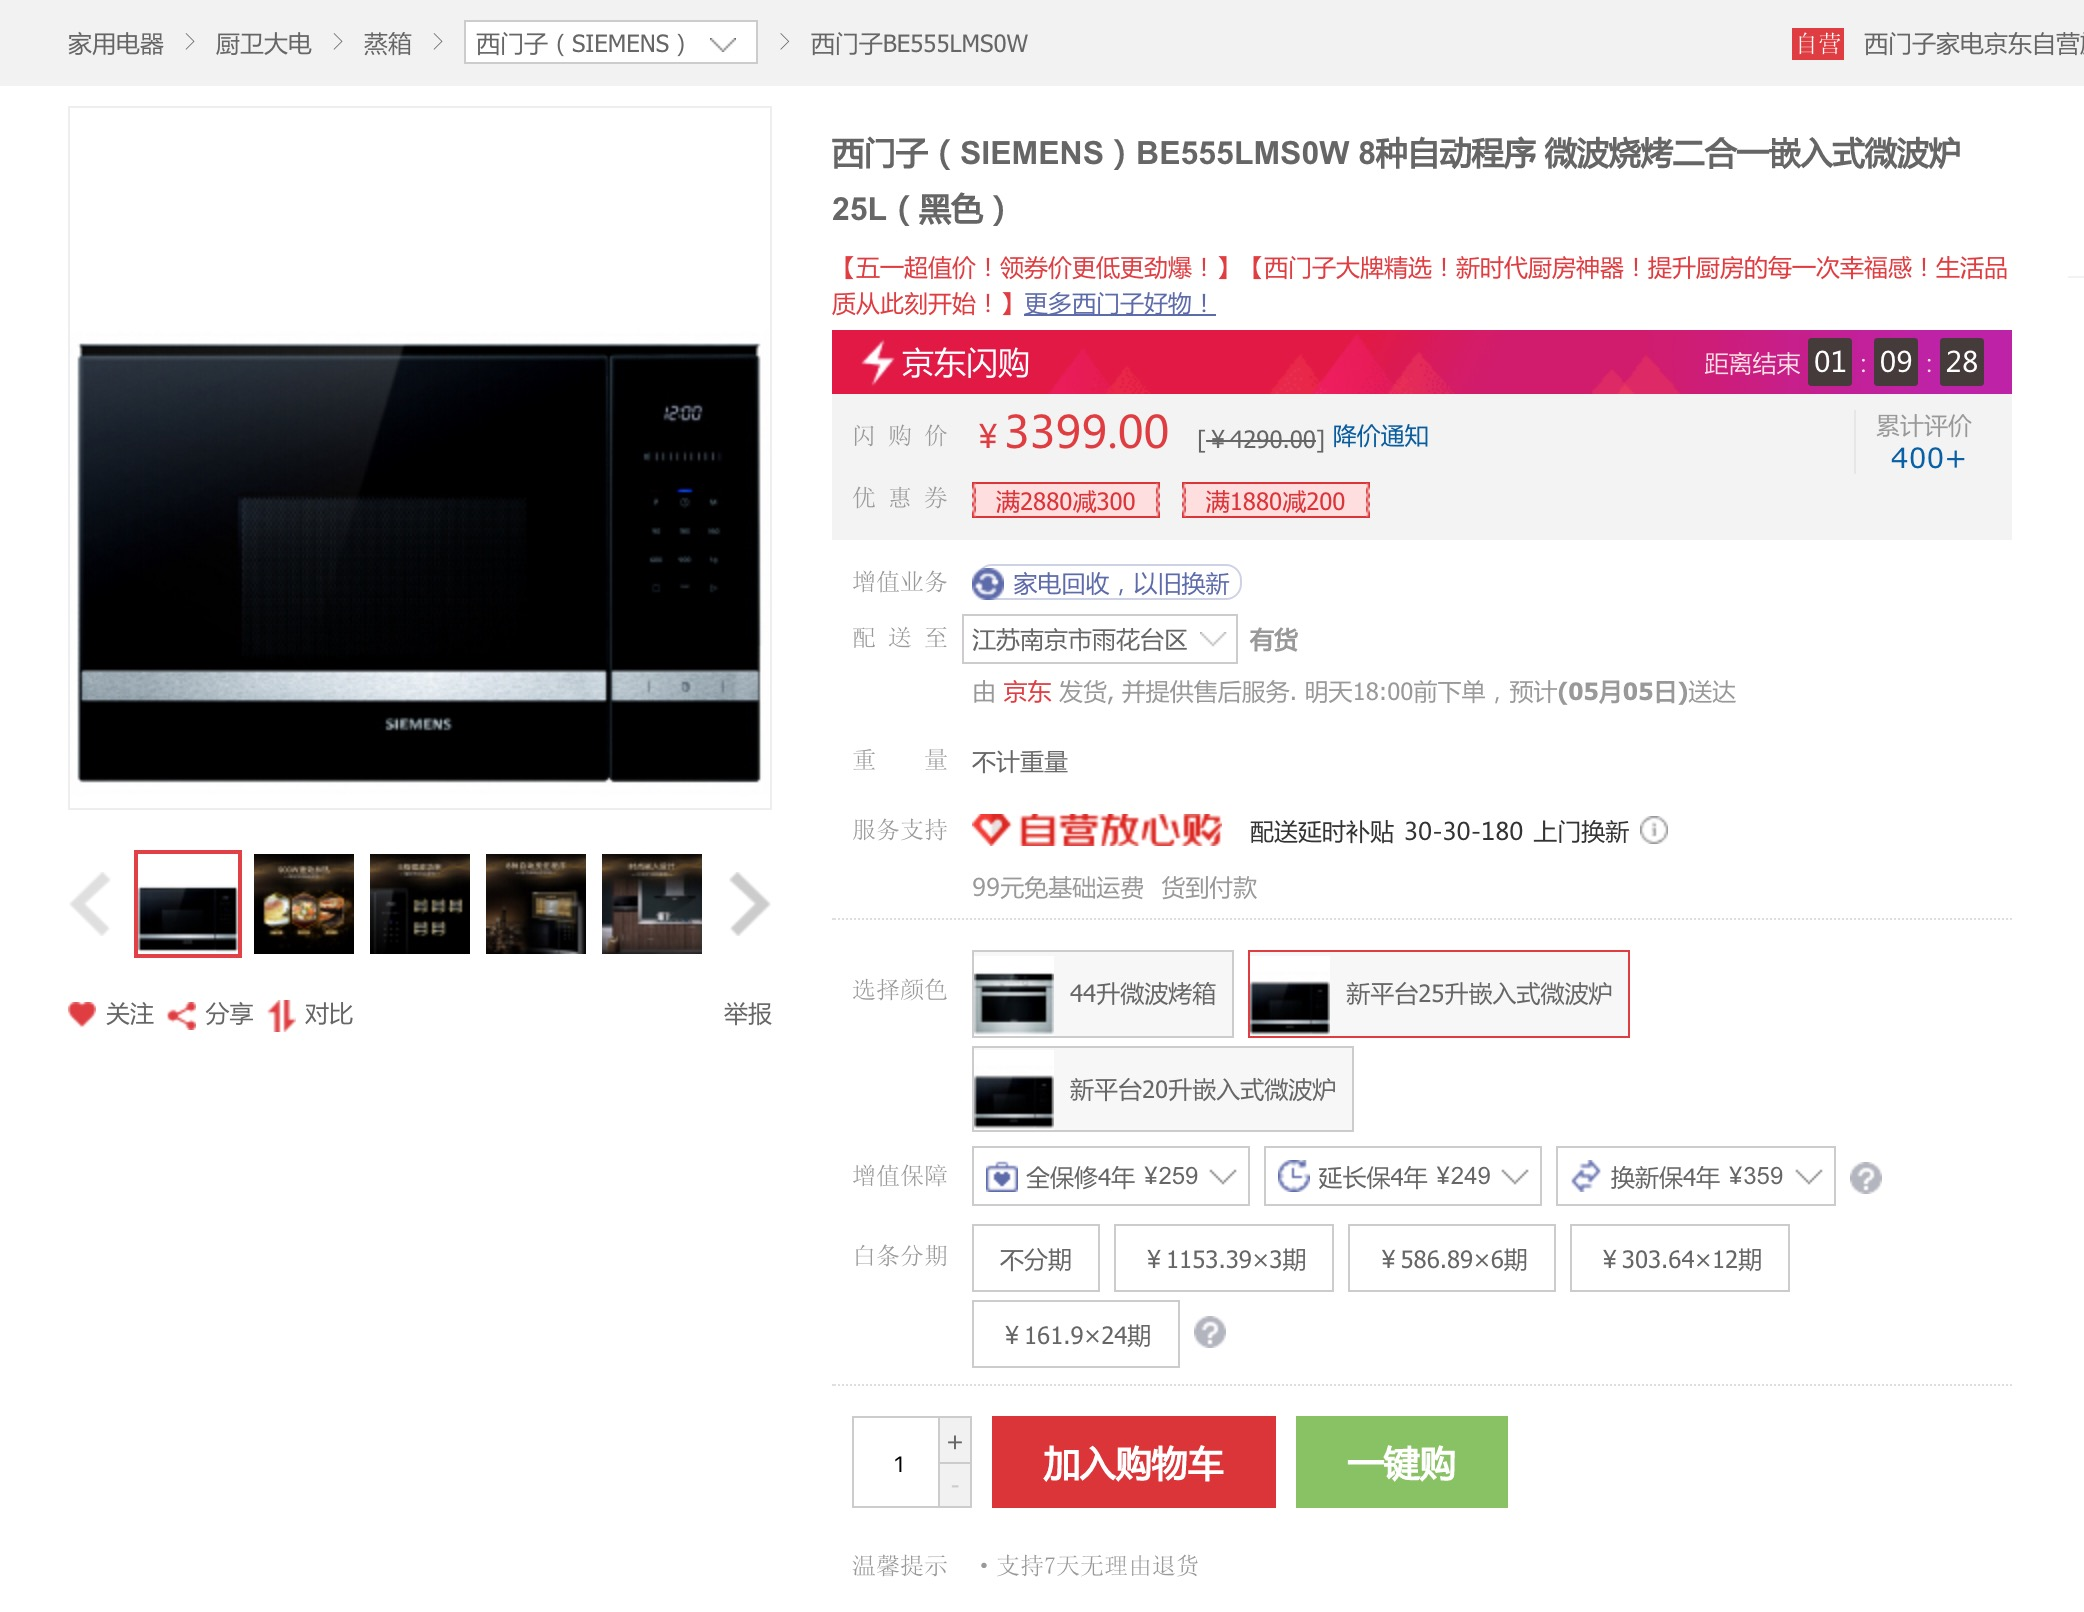
\includegraphics{/images/kaoxiang-simens3.jpeg}}

\begin{itemize}
\tightlist
\item
  厨余垃圾处理器
\end{itemize}

\href{https://detail.tmall.com/item.htm?spm=a220m.1000858.1000725.1.7f8c5e99l86tSK\&id=566529221807\&areaId=320100\&user_id=3048822382\&cat_id=2\&is_b=1\&rn=f2b270b27be73f2b5f17631edae39b3a}{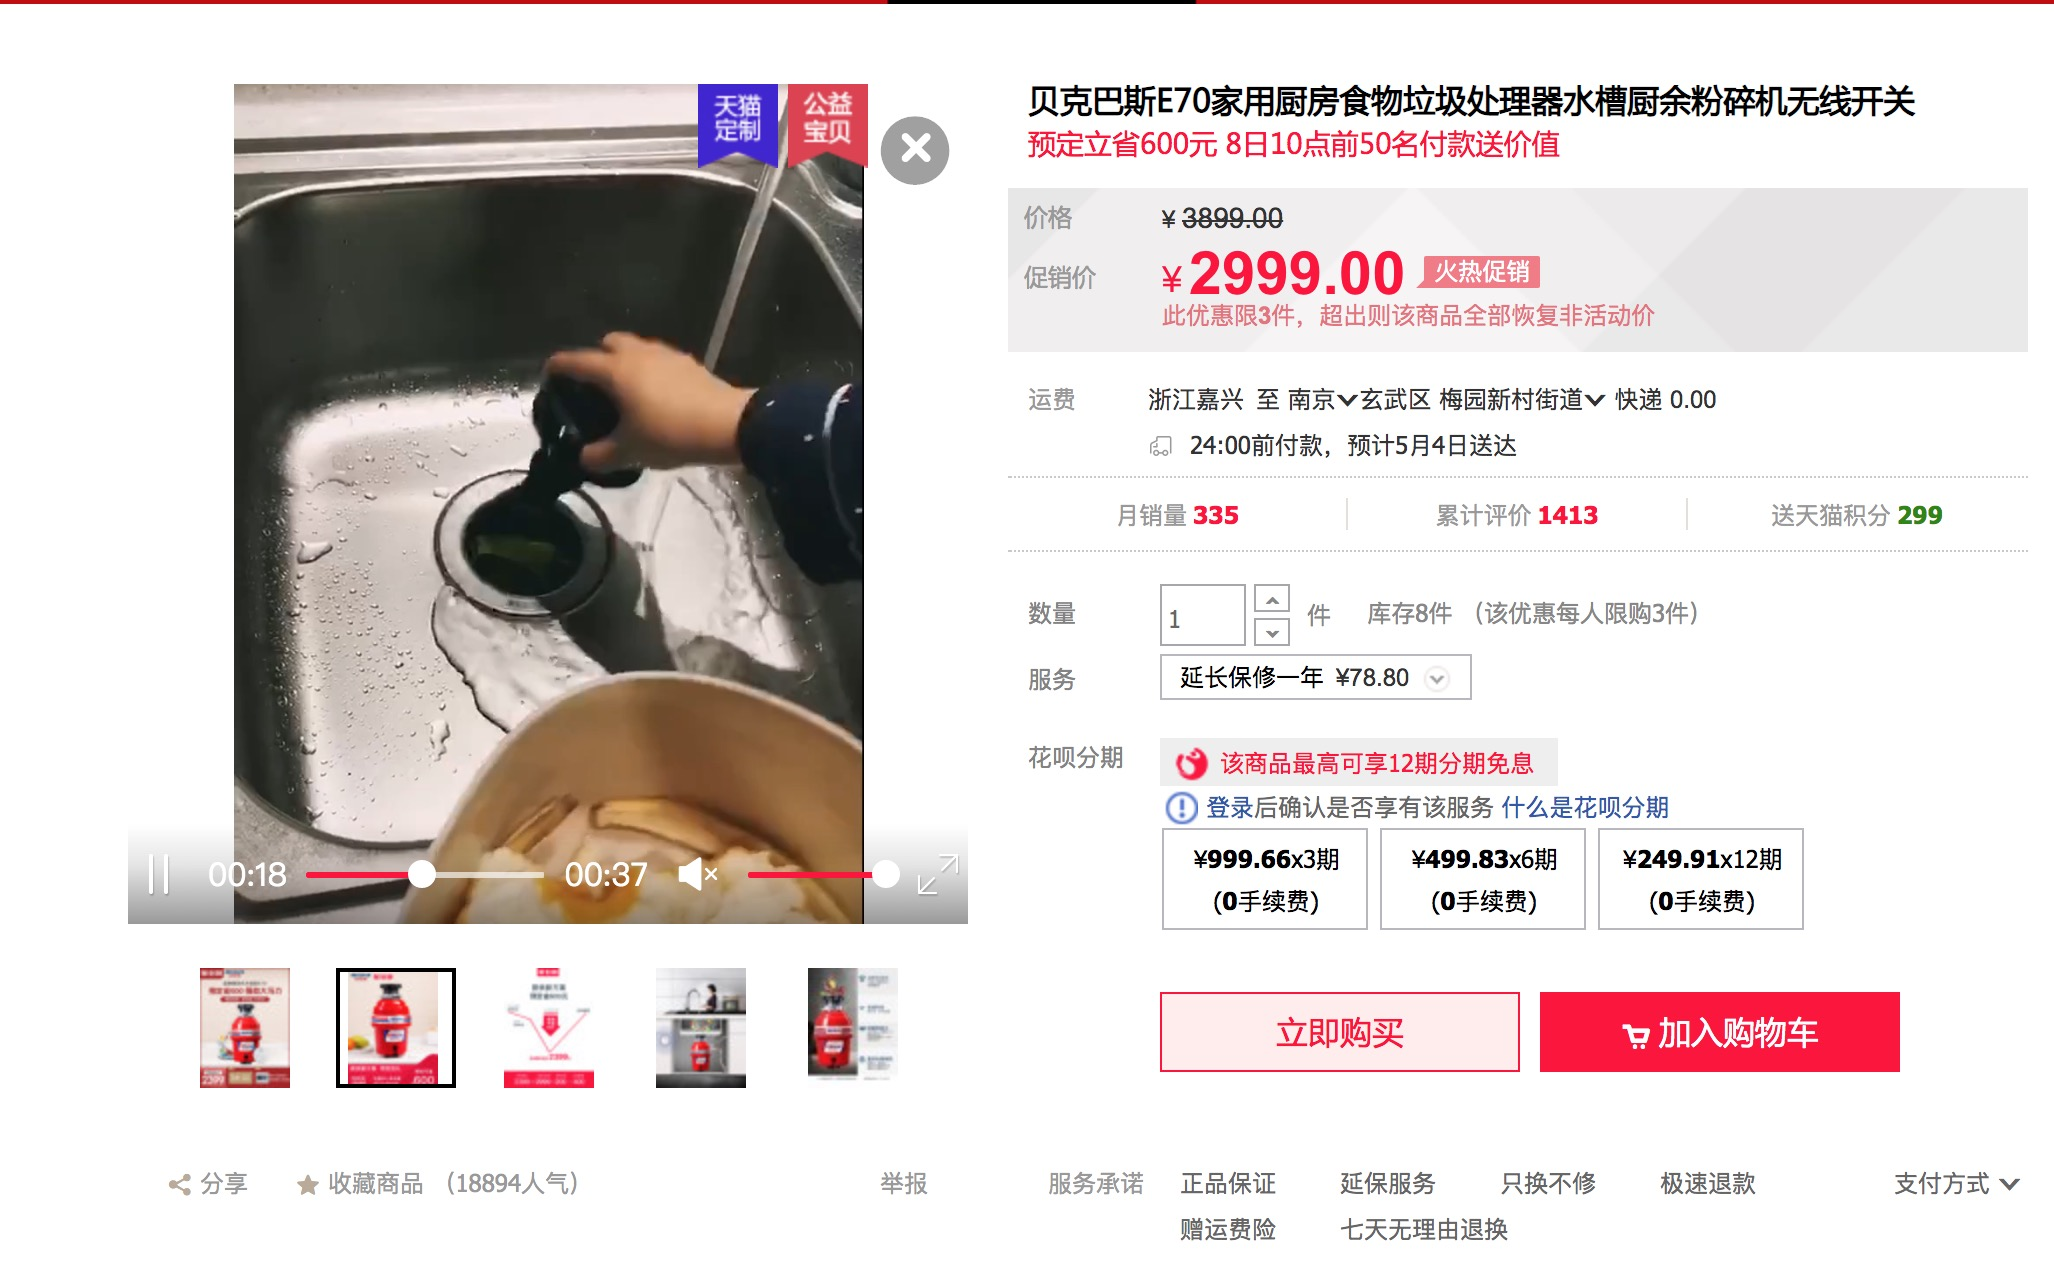
\includegraphics{/images/becbas1.jpeg}}
\href{https://detail.tmall.com/item.htm?spm=a1z10.3-b-s.w4011-15655300821.32.57ab46ddCA3nd1\&id=584865105801\&rn=7ce2caca976b3a87f4b8734c527aff17\&abbucket=3}{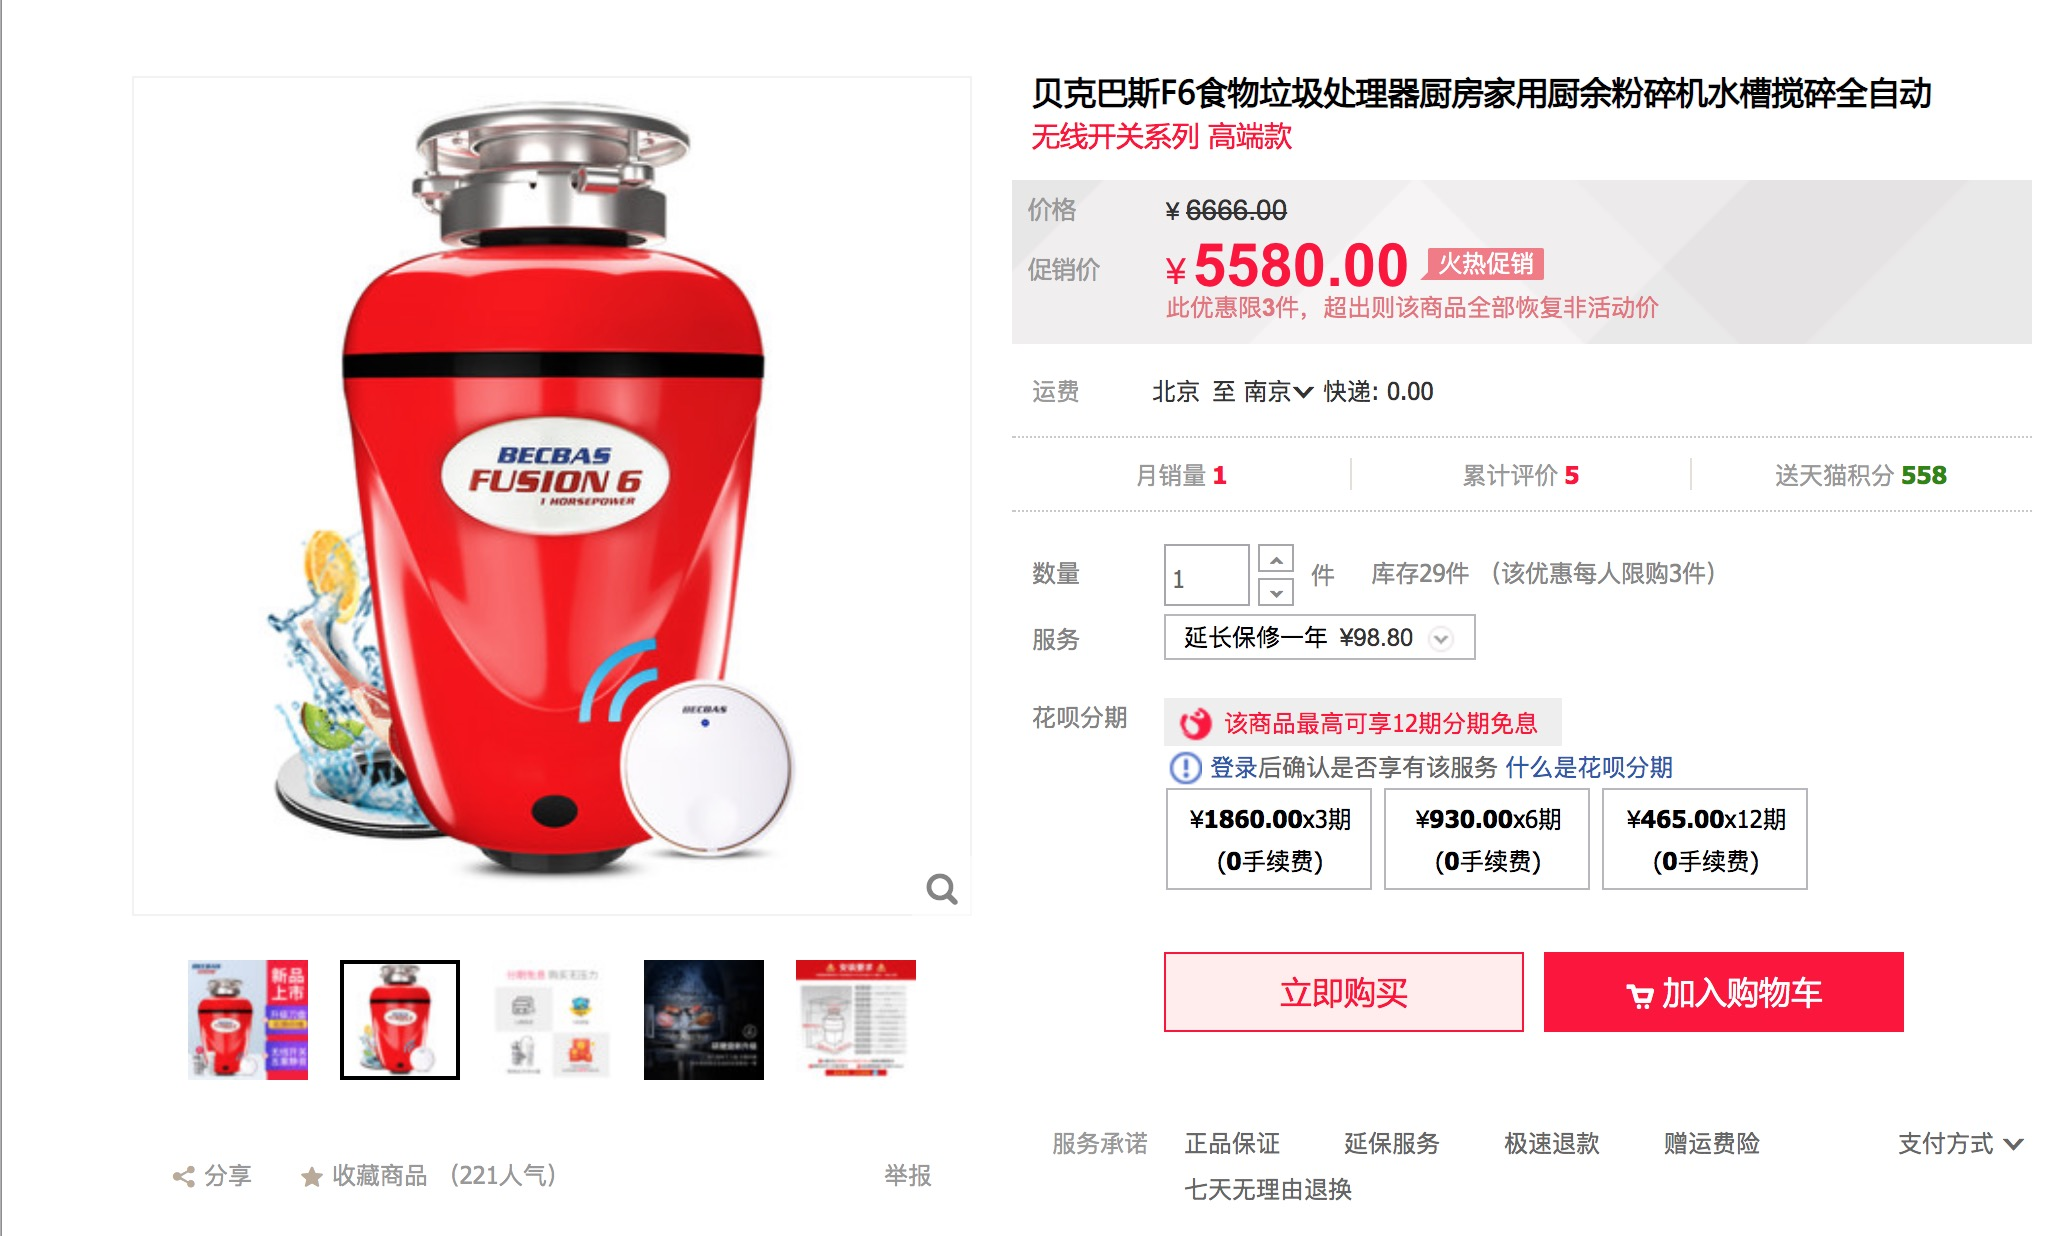
\includegraphics{/images/becbas2.jpeg}}

\paragraph{3.3 干衣机}

\href{https://item.jd.com/100002979925.html\#crumb-wrap}{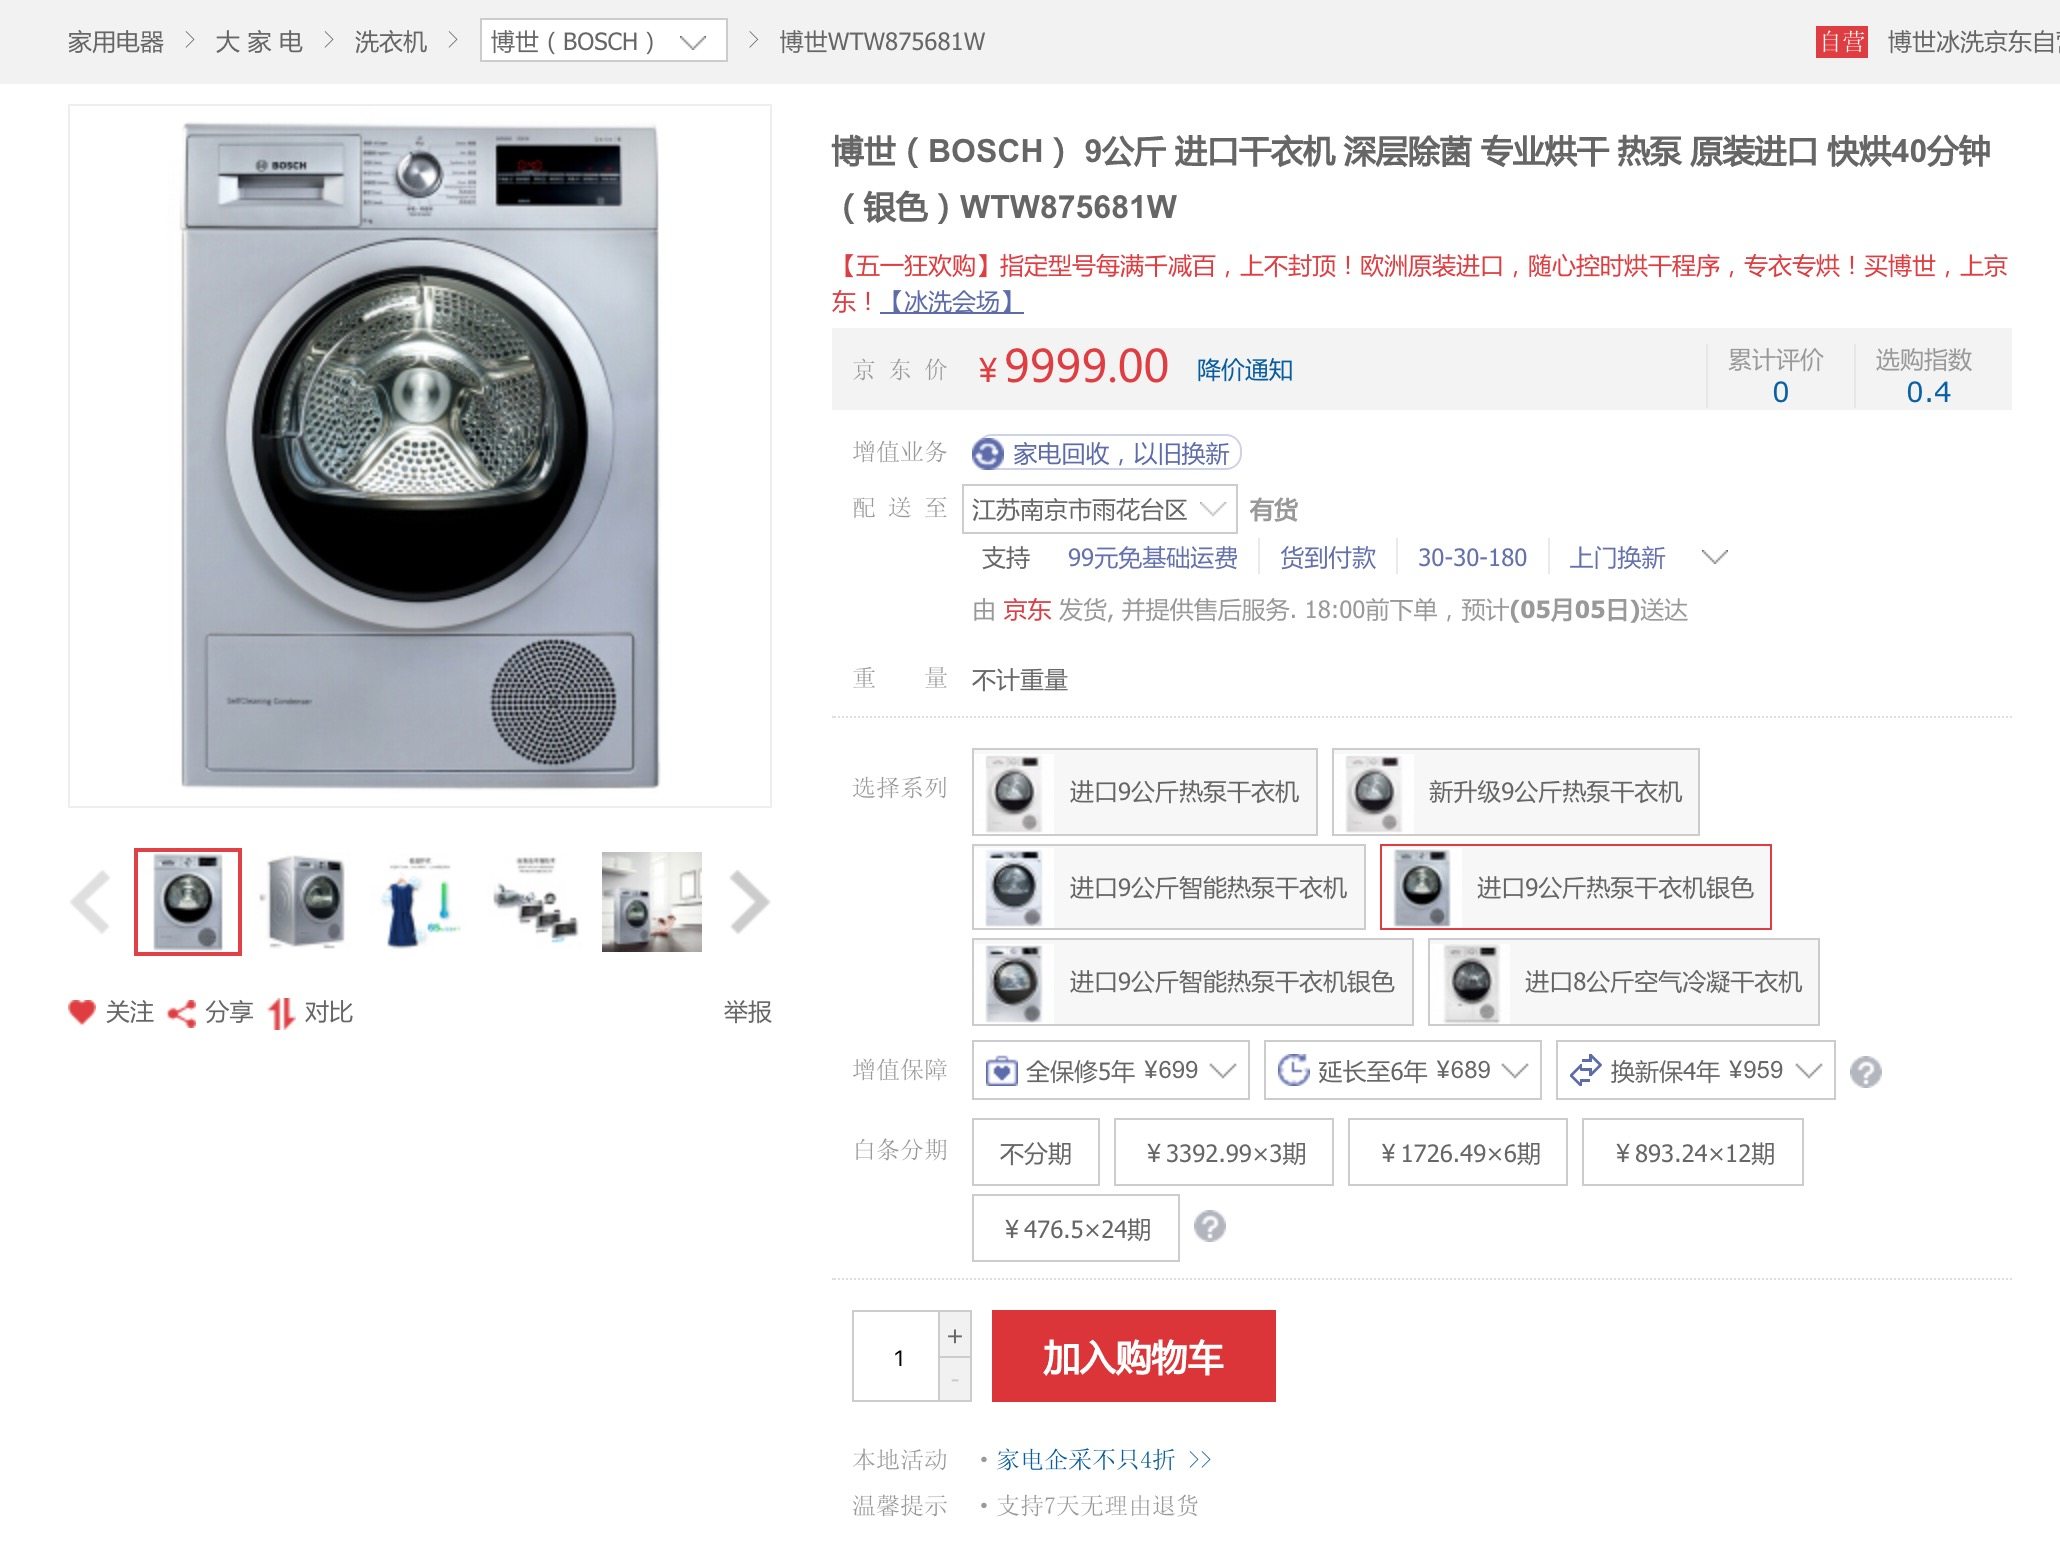
\includegraphics{/images/ganyiji.jpeg}}

\paragraph{3.4 卫生间电器}

\begin{itemize}
\tightlist
\item
  淋浴花洒
\end{itemize}

\href{https://item.taobao.com/item.htm?spm=a230r.1.14.15.75174969uHjSCl\&id=557954573996\&ns=1\&abbucket=16\#detail}{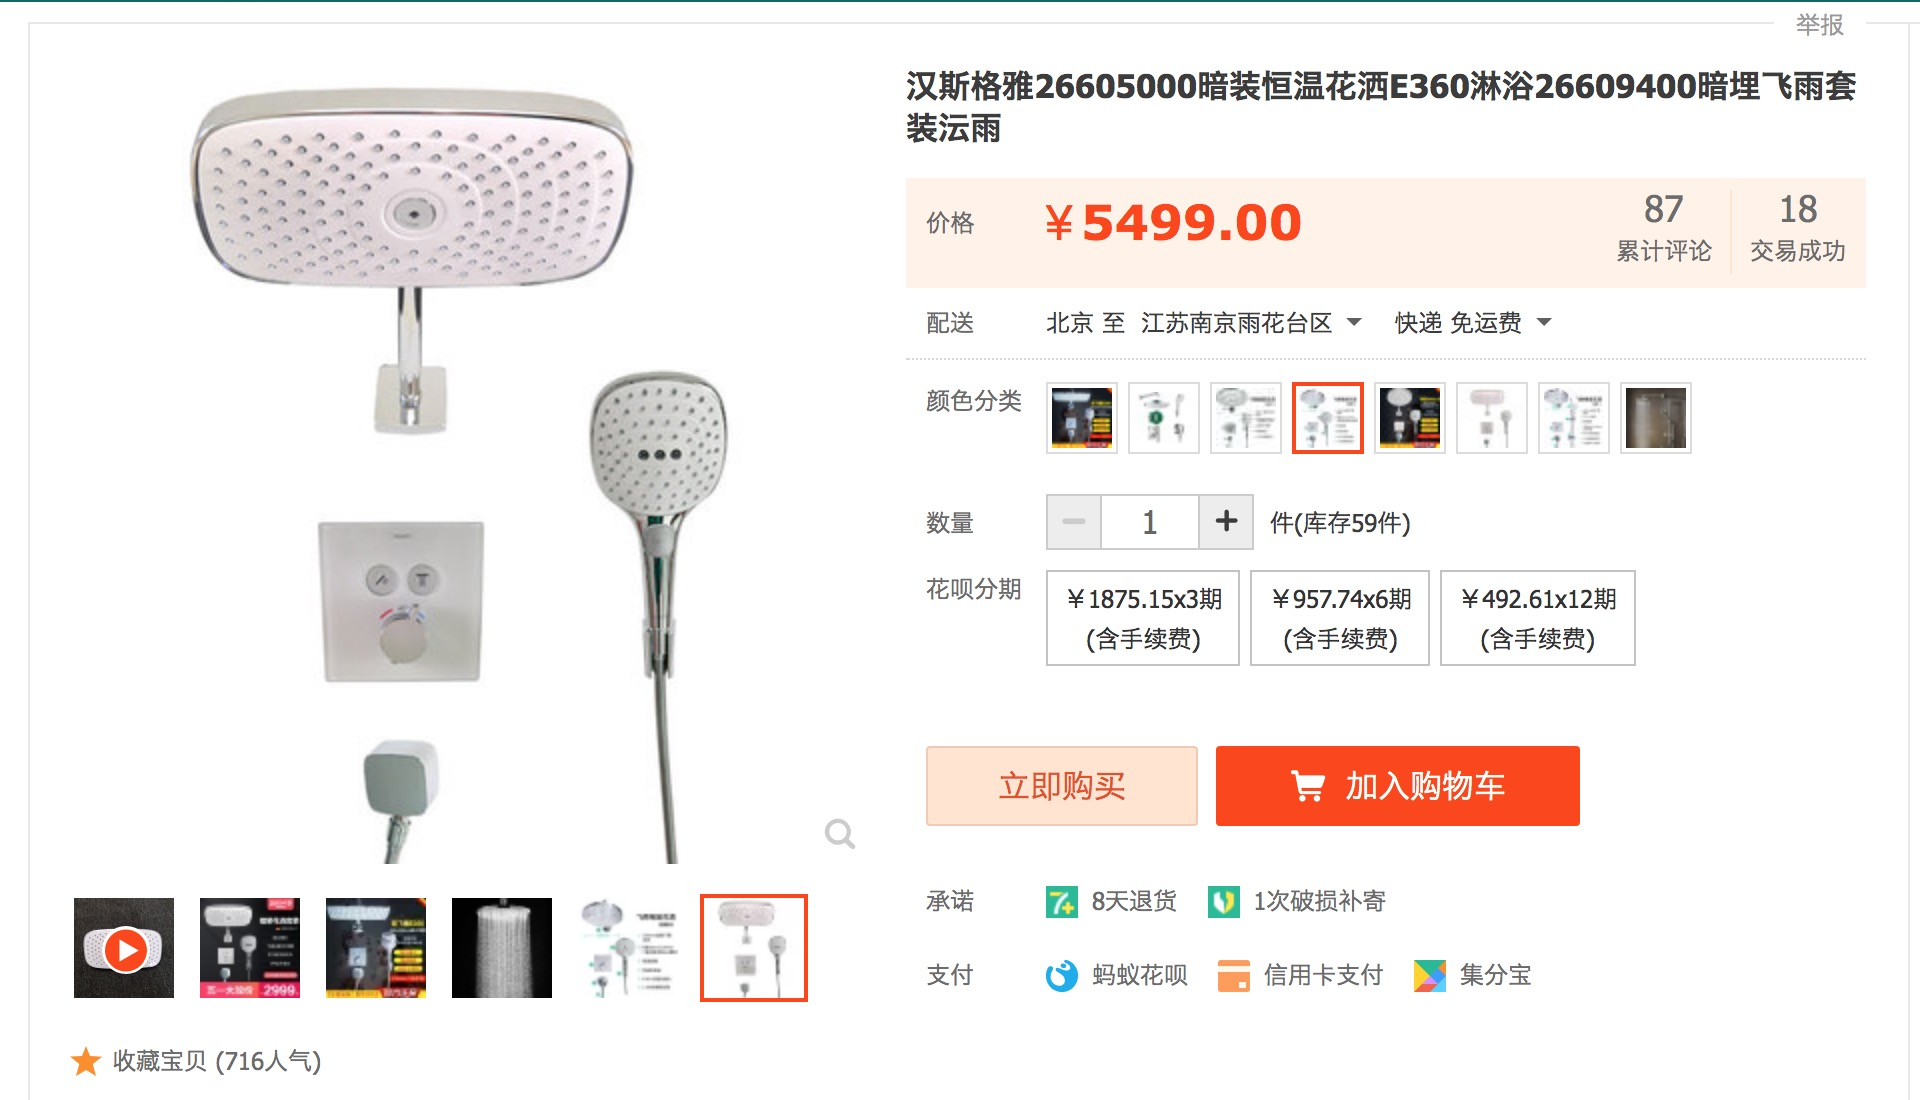
\includegraphics{/images/linyu-hans1.jpeg}}


\end{document}
